
\documentclass[UTF8,12pt]{ctexart}

    \setCJKmainfont{宋体}  
    \setCJKsansfont{黑体}  
    \setCJKmonofont{楷体}   
    \usepackage{setspace}  
    \setstretch{1.2}       
    \setlength{\parskip}{1em}  
    \newcommand{\upcite}[1]{\textsuperscript{\cite{#1}}} 
    \usepackage[toc, page]{appendix} 
    \renewcommand{\appendixtocname}{附录}
    \renewcommand{\appendixpagename}{附录}
    \usepackage{enumitem}   

    \usepackage{fancyhdr}    
    \pagestyle{fancy}         
    \fancyhf{}
    \usepackage{geometry}                
        \geometry{a4paper} 
        \geometry{hcentering}
            \chead{“深圳杯”数学建模挑战赛}   
            \rhead{\thepage}
            \renewcommand\headrulewidth{0pt}
    \usepackage{graphicx}           
    \usepackage{float}
    \usepackage{caption}
    \usepackage[export]{adjustbox}  
    \captionsetup[figure]{name=图片} 
    \usepackage{float}     
    \usepackage{booktabs}      
    \usepackage{longtable}     
    \captionsetup[table]{font=large}

    \usepackage{amsmath}     
    \usepackage{esint}         
    \usepackage{unicode-math}    

    \def\dif{\mathop{}\!{}\mathrm{d}}

    \usepackage{caption} 
    \usepackage{listings}



\begin{document}
\begin{titlepage}  %封面
    \centering
    \vspace*{\stretch{0}}{
        \huge{
            \textrm{
                2019\textbf{年“深圳杯”数学建模挑战赛}\\
                \ \\
                B\textbf{题}\\
                \ \\
                \ \\
                \ \\
                \textbf{新一代通信网络设计与规划}
            }
        }
    }\\

    \vspace{\stretch{2}}{
        \ \\
        \ \\
        \ \\
        \ \\
        \ \\
        \begin{align*}
            \text{\zihao{-2}中山大学:}\ \ &\text{\zihao{-2}林天皓}\\
            &\text{\zihao{-2}龙行健}\\
            &\text{\zihao{-2}卢浩文}
        \end{align*}
        }\\

    \vspace{\stretch{3}}
    {\today}
\end{titlepage}
%目录
\tableofcontents
\newpage
\section*{}%摘要
    \zihao{2}
    \centerline{\textsf{摘\ \ \ \ 要}}
    \zihao{-4}
    本文研究的是相控阵列天线的配置方式和骨干网的构建,针对前者,我们将所给天线量化,
    建立波束配置方式效用评价模型和区域覆盖效用评价模型;针对后者,
    我们建立了城市网络需求量评估模型,
    网络传输性价比评价模型和网络传输格式选型优化模型。\par
    针对微波问题一,通过分析目标方向上天线信号矢量的叠加结果,
    得到天线信号关于波束不同配置方式的函数方程,
    建立波束配置方式效用评价模型作为遗传算法的适应度参数,
    运用遗传算法搜索得出一种较优的矢量配置方式优的矢量配置方式$Z_1^{T}$。\par
    针对微波问题二,基于微波问题一波束配置模型,我们构建了区域覆盖效用评价模型,
    得到区域平均功率$M$和凹坑大小$D$关于不同配置方式的函数方程,同时,
    将其作为遗传算法的适应度参数,用算法搜索得出结果$Z_2^{T}$。\par
    针对骨干网问题一,先通过分析全国人均流量年际变化,
    运用回归分析方法估计2028年广东省全省流量为$150.4Tb/s$。
    根据广东省各个城市的人均可支配收入,平均年龄,人口数量,
    运用层次分析法建立城市评分模型估计各个城市未来流量需求量。
    结合城市位置和所需流量,运用最小生成树和蚁群算法找到一种网络构建方法。
    在确定网络构建方法后,建立网络传输格式选型优化模型,运用遗传算法和最大流算法,
    找到了成本为$1439.5X$满足全省流量的网络建设方法。\par
    针对骨干网问题二,建立了网络传输选型性价比函数,
    通过对每个覆盖率下成本最小的选型方式回归分析,得到了覆盖率与最小成本的拟合方程,
    取得性价比函数与覆盖率的关系,当性价比最大时,覆盖率为$75\%$.\par

\textsf{关键词:天线覆盖\ 骨干网部署\ 遗传算法\ 回归分析\ 层次分析法}
\newpage



\section{问题分析}
    \subsection{微波问题1}分析题目可知,
        我们的相控阵天线由32个天线组成,每一个天线能发出相对独立的波束,
        这些波束之间互相叠加与干涉,最终我们的相控天线总体的信号是这些波束互相叠加与干涉之后的结果。
        由此,我们建立单点功率计算模型,计算所有天线在区域内单点处的功率。
        然后对这32根各有5种移相器配置方式(包括关闭波束)的天线找到一种
        波束配置方式,使得叠加这些波束,发出的信号在水平角$AZ = 10°$,
        俯仰角$EL= 5°$的方向上合成功率大于$35dBm$,同时为了避免对在位置$AZ=10°$,
        俯仰$EL=10°$站点的干扰,需要发出的信号在水平角$AZ=10°$,
        俯仰角$EL=10°$的方向上的合成功率尽可能小,为了避免减小旁瓣,
        还要求其他方向的合成功率尽可能小。为了对这三个目标进行了量化分析,
        建立了波束配置方式效用评价模型。由于配置方式种类多达$5^{32}$种,
        传统的遍历式搜索无法在有限时间内给出一个最优解,
        而遗传算法非常善于解决这种搜索空间庞大,目标明确的问题,
        所以我们选择使用遗传算法求解。

    \subsection{微波问题2}
        与上题不同的是,该题不是要求单个方向的合成功率达到$35dBm$,
        而是在共有$91$个方向的一片区域上的平均功率达到$35dBm$,
        其次为了保证接收机在这片区域上的信号强度相对稳定,
        凹坑尽可能小——即在这片区域上信号功率的极差尽可能小,
        同时关闭尽可能多的天线加快扫描速度。针对这三个目标,我们需要对这些问题量化,
        同时建立区域覆盖效用评价模型,鉴于该问题的搜索空间与微波问题一相同,
        我们继承了问题一采用的遗传算法搜索一种使得评价函数值尽可能大的配置方式。
\newpage
    \subsection{骨干网问题1}
        题目给出,未来用户数据需求量呈指数形式的增长,
        需要对骨干网改造满足未来的要求。首先,我们需要建立数据需求模型、
        城市评分模型、评估2028年各个城市的信息需求量
        (由于题目假设需求量呈指数形式的增长,所以,只要满足2028年的需求,
        之前年份的需求也一定能被满足)。其次,需要解决如何构建网络和网络
        选用哪一种传输格式的问题,如何构建网络需要考虑线路最大传输距离和城市
        所需要流量的大小,而选用何种传输格式,多少根线的问题,这涉及到成本的考虑。
        题目附件给出传输容量为$800Gb/s$的线路每$Gb/s$的相对成本最低,
        但是最大传输距离最短,所以,距离在$80km$以内的线路都采用这一种线路。
        最后,我们需要寻找满足全部需求的情况下成本最小的路线部署位置及铺设光纤数。
        整合线路选择、路线部署位置与铺设光纤数,就是我们要找的网络建设部署方案。

    \subsection{骨干网问题2}
        对于该题,可以不需要满足整个网络的需求,要取得效益最大的网络建设效果。不难估计,
        建设骨干网络是一个边际效益递减的工程,
        覆盖最后百分之十的成本一定比覆盖前百分之十的成本要高,
        所以我们设定骨干网络建设效率函数评估当前选定的网络建设方式,成本尽可能低,
        覆盖率(当前网络建设下满足的流量/全省流量)尽可能大。对于这个二元函数,
        我们逐个参数考虑,先考虑覆盖率一定时候成本最低是多少,
        接下来找到性价比(覆盖率/成本)最高的点,得到接入网络价值最大的部署方案。
        
        


\newpage
\section{模型假设}\label{mxjs}
    \subsection{微波问题}
        \begin{enumerate}
            \item 假设微波接收机在无穷远处,即微波接收机与所有阵列天线的角度相等
            \item 在所给的测量数据中,相控天线每$5°$给出一组实际测量数据,我们以其数据
                代表其附近$2.5°$区域内的信号强度和相位。
            \item 功率与相位实际测量数据中的空数据($inf$和$nan$数据)均视为0进行处理
        \end{enumerate}
    

    \subsection{骨干网问题}
        \begin{enumerate}
            \item 各个城市、人群的实际数据需求量总体随时间递增,但它并不是随时间一直增加的——
                例如,每一天,用户带宽需求都会随着时辰的改变而改变。
                信息网络的部署实际上应该着眼于每天/每周的用网高峰期。
                则在本文中,我们讨论的“数据需求量”均表示每天/每周用网高峰期的实际数据需求量。

            \item 骨干网承担各城市对外网络交互的出入口功能,起止点应该设于各个城市中心
                我们合理地假设所有光缆铺设的起止点位于各个城市的市政府附近,并以各市市政府
                位置为标准测量各城市间的距离。
            
            \item 光缆的铺设与维护是一项专业性工作,不需要像铺设公路考虑驾驶员安全一样苛刻。
                在铺设光缆时,只需要避开极端地形。不考虑海拔变化/地形因素对光缆长度的影响,
                我们合理地假设在两城间铺设光缆时,成本最低的方案大致为全线沿直线铺设。依此,
                一并假设光缆的成本仅由起止点、线路类型、光缆中光纤数目决定。且不考虑光缆的铺设时间。
            \item 假设未来用户数据需求量呈指数形式的增长。
            \item 假设广东省各城市未来十年人口基本不变。
            \item 由于潮汕三市——汕头、揭阳、潮州所选基点(市政府)距离极小,可以确定
                最佳连接方案就是广州—……—揭阳,揭阳—汕头,揭阳—潮州。则在构建蚁群算法模型和
                最小生成树模型时,将潮汕三市作为一个整体考虑
        \end{enumerate}


\section{符号说明}
    \subsection{微波问题}
        \begin{enumerate}
            \item $k$ :单天线的五种配置方式,取值为$0,1,2,3,4$,
            分别代表该天线:关闭$,$位移$0°,90°,180°,270°$
            \item $\overrightarrow{e_i}$ :单个天线在区域中某点产生的信号矢量
            \item $w_i$ :单个天线在区域中某点产生的功率强度
            \item $\overrightarrow{E_i}$ :32个天线在区域内某点叠加后的矢量
            \item $|\overrightarrow{E_i}|$ :32个天线在区域内某点叠加后的矢量强度
            \item $\varphi_{ik}$ :单个天线在区域内某点的配置方式下相位大小,k在此处不等于0
            \item $G_v$ :目标点功率值
            \item $I_v$ :干扰点功率值
            \item $O_v$ :单个个体的适应值
            \item $K$ :旁瓣功率大小,即除了目标点功率之外其余点中功率最大的值
            \item $D$ :凹坑的功率大小,即全局最大最小值之差;
            \item $C$ :波束关闭的数量;
            \item $W = 20\cdot log_{10}{|\overrightarrow{E}|}$:功率和信号强度的转化公式
        
       
        \end{enumerate}
    
    \subsection{骨干网问题}
      \subsubsection{数据需求模型}
        \begin{enumerate}
            \item $O$层:数据需求的层次结构中的目标层,即数据需求量。
            \item $C$层:数据需求的层次结构中的准则层,包括了商业需求、个人需求、行政需求。
            \item $D$层:数据需求的层次结构中的决定层,包括了年龄、收入、人口。
            \item $A_{X-Y}$:$X$层的所有元素对上一层$Y$元素之影响的成对比较矩阵
            \item $\lambda _{max}$:
                成对比较矩阵的最大特征值(或其组成的向量)
            \item $\overrightarrow\omega _{C-O}$:
                $A_{C-O}$的最大特征值所对应的特征向量,称为权向量
            \item $W_{D-C}$:$A_{D-C_1},A_{D-C_2},A_{D-C_3}$的最大
                特征值分别对应的特征向量组成的矩阵,称为权向量矩阵
            \item $n_{x-y}$:进行成对比较的元素数目
            \item $CI_{X-Y}$:层次分析中的一致性指标
            \item $RI_{X-Y}$:层次分析中的平均随机一致性指标
            \item $CR_{X-Y}$:层次分析中的随机一致性比率
        \end{enumerate}
      
      \subsubsection{城市评分模型}
        \begin{enumerate}
            \item $C_k$:城市k
            \item $Y_k$:城市k的平均年龄
            \item $x_{k1}$:城市k的年龄得分
            \item $I_k$:城市k的人均可支配收入
            \item $x_{k2}$:城市k的收入得分
            \item $P_k$:城市k的人口
            \item $x_{k3}$:城市k的人口得分
            \item $x_k$:城市k的(加权后)总得分
            \item $N_k$:城市k的数据需求量
        \end{enumerate}

      \subsubsection{蚁群算法模型}
        \begin{enumerate}
            \item $n$:城市数量
            \item $u_{k_1k_2}$:城市$k_1,k_2$的距离
            \item $N_k$:城市k的数据需求量
            \item $N_{k_1k_2}$:城市$k_1,k_2$的数据需求量之和
            \item $a$:蚁群算法信息素权重参数
            \item $b$:蚁群算法原始权重参数
            \item $c$:蚁群算法信息素挥发速度参数
            \item $d$:蚂蚁走过路线时该线路增加的信息素含量
            \item $s$:蚂蚁种群数量
            \item $P_i$:蚂蚁向其他城市移动的概率向量
            \item $T_{ij}$:城市$k_i,k_j$之间路线的信息素含量
        \end{enumerate}
      \subsubsection{最小生成树模型}
        \begin{enumerate}
            \item $n$:城市数量
            \item $u_{k_1k_2}$:城市$k_1,k_2$的距离
            \item $N_k$:城市k的数据需求量
        \end{enumerate}
      \subsubsection{网络传输格式选型评价模型}
        \begin{enumerate}
            \item $Req$:全省所需要的网络流量
            \item $Cost$:建设网络所需要的标准成本
            \item $W$:网络对全省网络需求的满足率
            \item $f_K$:当前配置方式下全省最大允许的网络流量
            \item $L$:网络传输格式设置向量,长度21
            \item $K$:每条路径采用的网络线路数量向量,长度21
            \item $C$:每条路径网络流量容量向量,长度21
            \item $l_i$:第i条路径的传输格式设置
            \item $d_i$:第i条路径的距离
            \item $k_i$:第i条路径采用的网络线路数量,由附件可知最大为80
            \item $c_i$:第i条路径网络流量容量;
            \item $K_m$:由遗传算法计算得出的最优网络线路数量向量
        \end{enumerate}
      \subsubsection{网络传输性价比模型}
        \begin{enumerate}
            \item $W$:网络对全省网络需求的满足率
            \item $f_K$:当前配置方式下全省最大允许的网络流量
            \item $K$:每条路径采用的网络线路数量向量,长度21
            \item $E(K)$:当前配置方式下的网络性价比
        \end{enumerate}

\newpage

\section{模型建立}
    \subsection{单点功率计算模型}
    考虑天线阵列在半球面上产生的功率状况,将半球面展开成平面,
    在欧几里得平面几何中进行运算,因为题目给的数据为隔$5°$取一点,
    所以采用单点叠加代表一个$5°×5°$的区域面积功率大小。
    对于单个天线$u_i$,其在水平$(-180,180)$和垂直$(-90,90)$某点产生的功率
    $w_i$大小为:$$w_i = 20\, log_{10}{|e_i|}$$\par
    
    考虑对于单点矢量信号$E_i$,将其信号强度投影到x轴和y轴上,则
    $$\vec{e_{ix}} = \vec{e_{i}}×cos(\varphi_{ik}), \quad 
    \vec{e_{iy}} = \vec{e_{i}}×sin(\varphi_{ik})$$\par
    
    对于单个天线区域内单点的合信号$\vec{E_{i}}$,其计算公式为
    $$\vec{E_{i}}=\sum_{1\leqslant i \leqslant 32} \vec{e_{i}}$$\par
    
    对于单个天线区域内单点的合信号的模$|E_i|$,由矢量的计算公式,得
    \begin{gather*}
        |\vec {E_{ix}}| = \sum_{1\le i \le 32} |\vec {e_{ix}}|\\
        |\vec {E_{iy}}| = \sum_{1\le i \le 32} |\vec {e_{iy}}|\\
        |\vec {E_i}| = \sqrt{|\vec {E_{ix}}|^{2}+|\vec {E_{iy}}|^{2}}
    \end{gather*}\par
    最后,可得所有天线在区域内单点处的功率
    $$W_i = 20\, log_{10}{|E_i|}$$


    \subsection[适应度模型1]{适应度模型1——波束配置方式效用评价模型}\label{SYDY}
        为了量化遗传算法中的适应值,起到评价单个个体在种群中的竞争地位的目的,
        我们选用单个个体波束配置方式的效用模型作为其适应度的参考值,模型的构建如下:
        \begin{Large}
            $$Ov = \underbrace{\frac{1}{1+e^{-(Gv-a)b}}}_{\text{Ov-weight}}×\underbrace{c\, e^{(\frac{d-Iv}{f})}}_{\text{Iv-weight}}×\underbrace{{K}^{-μ}}_{\text{K-weight}}$$
        \end{Large}
        其中$a,b,c,d,f,μ$分别是该模型中$Gv$和$Iv$可以调整的权重参数,
        在问题的求解中可以通过调整达到较优化的结果。\par

        \noindent 该模型由三部分组成:\par
        第一部分是目标点功率值,即$Ov$的权重,我们采用$sigmol$函数来配比,
        其目的是为了筛选出题目硬性要求的目标点功率值在35dbm以上的个体,
        使得他们在种群中的竞争优势大大增加。\par
        第二部分则是干扰点的功率值,即$Iv$的权重,我们采用指数函数,
        因为其快速增长特性可以帮助我们在同等$Gv$条件下扩大较小$Iv$的优势。\par
        第三部分是旁瓣的大小,即除了目标($10°,5°$)
        之外其余坐标中最大的点的功率值,我们给其分配一个负幂指数,
        使得其越小对于整体的函数值贡献却越大。

\newpage
    \subsection[适应度模型2]{适应度模型2——区域覆盖效用评价模型}\label{SYDE}
        为了量化遗传算法的适应值函数,我们再次构建模型,
        考虑区域每个配置方式下对指定区域的平均功率、凹坑和天线关闭个数进行量化计算。\\
        水平$(-30°,+30°)$,竖直$(-15°,+15°)$区域共91个点的平均合成功率$M$为:
        $$M = \frac {\sum{W_i}} {91}$$
    
        \noindent 凹坑$D$的计算公式为:
        $$D = Max(W_i)-Min(W_j)$$
    
        \noindent 则可以得出适应度的计算方法为:
        \begin{Large}
            $$Ov = \underbrace{e^{-\frac {D}{a}}}_{\text{D-weight}}×\underbrace{(C+σ)}_{\text{C-weight}}× \underbrace{\frac {1}{1+e^{-(M-d)f}}}_{\text{M-weight}}$$
        \end{Large}
        其中$a,σ,c,d,f$分别是该模型中凹坑、关闭波束数量、
        区域平均功率强度的权重参数。\par
        
        \noindent 模型的构建分为三部分:\par
        第一部分是凹坑的权重配置,我们用指数函数来最小化凹坑的值。\par
        第二部分是关闭天线个数的权重,在这种情况下采用线性的函数来调整其权重,
        使得其值的变化有影响但是不是特别重要。\par
        第三部分也是采用$sigmol$函数来配重,再次利用了其优良的徒增特性,
        起到很好的筛选作用。

    \subsection{数据需求模型}\label{ShuJv}
            \begin{figure}[H]
                    \centering
                    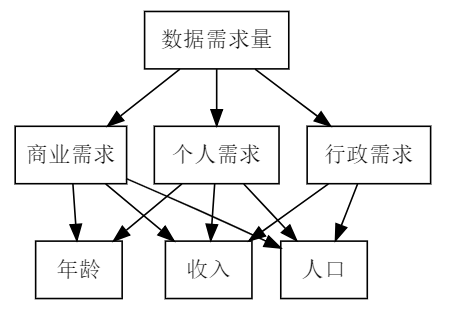
\includegraphics{need.png}
                    \caption{数据需求层次结构}\label{SJXQCCJG}
                \end{figure}
        为了判断各个影响因素对一座城市的数据需求量的影响权重,建立层次结构模型,如图片\ref{SJXQCCJG}。

        \begin{enumerate}
            \item C层对数据需求量的影响:
            \begin{enumerate}
                \item 建立成对比较矩阵:
                $A_{C-O}=\begin{bmatrix}
                    1 & \frac{1}{4} & 4 \\                    
                    4 & 1 & 8\\                  
                    \frac{1}{4} & \frac{1}{8} & 1
                 \end{bmatrix}$
                \item 求得最大特征值$\lambda _{max}=3.0536$及其对应的权向量为
                    $$\overrightarrow\omega_{C-O}=(0.2227,0.7071,0.0702)$$
                \item 由$n_{c-o}=3$,求得$A_{C-O}$的一致性指标$CI_{C-O}=0.0268$
                \item 由$n_{c-o}=3$,得平均随机一致性指标$RI_{C-O}=0.58$,
                    则随机一致性比率$CR_{C-O}=0.0462<0.1$,接受该层分析。\\
            \end{enumerate}
            则认为商业需求,个人需求,行政需求对数据需求量影响的比重分别为$0.2227,0.7071,0.0702$。
              
            \item D层对数据需求量的影响:
            \begin{enumerate}
                \item 为D层对商业需求的影响建立成对比较矩阵:
                $$A_{D-C_1}=\begin{bmatrix}
                    1 & \frac{1}{8} & \frac{1}{6} \\
                    8 & 1 & 1\\
                    6 & 1 & 1
                 \end{bmatrix}$$
                \item 为D层对个人需求的影响建立成对比较矩阵:
                $$A_{D-C_2}=\begin{bmatrix}
                    1 & \frac{1}{2} & \frac{1}{8} \\
                    2 & 1 & \frac{1}{7}\\
                    8 & 7 & 1
                 \end{bmatrix}$$
                \item 为D层对行政需求的影响建立成对比较矩阵:\\(其中$D_1$不影响行政需求)
                $$A_{D-C_3}=\begin{bmatrix}
                    1 & \frac{1}{2}\\
                    2 & 1
                 \end{bmatrix}$$
                \item \begin{itemize}
                    \item 求得这三个成对比较矩阵的最大特征值向量为$$\lambda _{max}=(3.0092,3.0349,2)$$
                    \item 其对应的权向量矩阵为$$W_{D-C}=\begin{bmatrix}
                        0.0672 & 0.0813 & 0 \\
                        0.4887 & 0.1349 & 0.3333 \\
                        0.444  & 0.7838 & 0.6667
                     \end{bmatrix}$$
                    \item 对应的D层对O层的组合权向量为$$\omega_{D-O}=\begin{bmatrix}
                        0.0672 & 0.0813 & 0 \\
                        0.4887 & 0.1349 & 0.3333 \\
                        0.444  & 0.7838 & 0.6667
                     \end{bmatrix}×\begin{bmatrix}
                        0.2227 \\
                        0.7071 \\
                        0.0702
                     \end{bmatrix}=\begin{bmatrix}
                        0.0725 \\
                        0.2276 \\
                        0.6999
                     \end{bmatrix}$$
                    \end{itemize}                    
                \item 则D层对C层的一致性指标为
                    $$CI_{D-C}=[0.0046,0.0174,0]×\begin{bmatrix}
                    0.2227 \\
                    0.7071 \\
                    0.0702
                     \end{bmatrix}=0.0133$$
                \item 又有D层对C层的平均随机一致性指标为
                    $$RI_{D-C}=[0.58,0.58,0]×\begin{bmatrix}
                    0.2227 \\
                    0.7071 \\
                    0.0702
                     \end{bmatrix}=0.5393$$
                \item 则D层对O层的组合随机一致性比率为
                    $CR_{D-O}=0.0462+\displaystyle\frac{0.0133}{0.5393}=
                    0.0709<0.1$,接受该层分析。
            \end{enumerate}

        \end{enumerate}
        综上,得到年龄,收入,人口对数据需求量影响的比重分别为$0.0725,0.2276,0.6999$
        


    \subsection{城市评分模型}\label{PingFen}
        \subsubsection{平均年龄评分}
            当今社会中的年轻人,特别是大学生使用互联网教多,数据需求量较大。
            数据需求量的峰值大约在年龄为15岁~25岁之间达到。
            广东省内各城市平均年龄均大于30岁,则年龄与数据需求量大致可视为负相关,
            则选择以反比例尺度对平均年龄评分
            \begin{itemize}
                \item 以广州市的平均年龄$Y_1=34.4$岁为100分
                \item 某市$C_k$的平均年龄为$Y_k$,满足$Y_1=\displaystyle\frac{x_{k1}}{100}·Y_k$,则该市年龄得分为$x_{k1}$
                \item 任一城市$C_k$的年龄得分为\begin{large}
                    $$x_{k1}=\frac{100Y_1}{Y_k}$$
                \end{large}
            \end{itemize}

        \subsubsection{人均可支配收入评分}
            数据需求量应当与收入呈正相关,但随着收入的增加,
            数据需求量的增长率不会一直保持水平,应该随收入的增加而逐渐降低。
            则选择以对数尺度对人均可支配收入评分:
            \begin{itemize}
                \item 以广州市人均可支配收入为100分\par 
                    (\ 设广州市人均可支配收入$I_1=5.5356=a^{100}$万元\ )
                \item 某市$C_k$的人均可支配收入$I_k=a^{x_{k2}}$万元,则该市收入得分为$x_{k2}$
                \item 任一城市$C_k$的收入得分为\begin{large}
                    $$x_{k2}=\log _{I_1}({I_k}^{100})=\frac{100\ln I_k}{\ln I_1}$$
                \end{large}
            \end{itemize}

        \subsubsection{人口评分}
            由于城市需求量大致是每个群体的群体需求量的总和,
            所以人口与数据需求量大致成线性关系。则选择以线性尺度对城市人口评分
            \begin{itemize}
                \item 以广州市的人口$P_1=1490.44$万人为100分
                \item 某市$C_k$的人口为$P_k$,
                    则该市的人口得分为\begin{large}
                        $$x_{k3}=\frac{100P_k}{P_1}$$
                    \end{large}
            \end{itemize}
    
    
    \subsection{蚁群算法模型}\label{YQSFMX}
        \begin{enumerate}
            \item 根据每两个城市之间的距离$u_{ij}$和
            每两个城市数据需求量之和$N_{ij}=N_i+N_j$,建立路径的原始权重邻接矩阵
            $$D_{ij}=\frac{N_{ij}}{u_{ij}}$$
            \item 创建信息素邻接矩阵$T$,大小与$D$相同
            \item 对$s$只每只蚂蚁随机选取城市$i$做为起点
            \item 对于每只蚂蚁,计算蚂蚁向其他城市移动的概率向量$P_i$
            \begin{large}
                $$P_i=\left[\frac{D_{i1}^bT_{i1}^a}{\sum_{k=1}^n{D_{ik}^bT_{ik}^a}}~\frac{D_{i2}^bT_{i2}^a}{\sum_{k=1}^n{D_{ik}^bT_{ik}^a}}~··· \frac{D_{in}^bT_{in}^a}{\sum_{k=1}^n{D_{ik}^bT_{ik}^a}}\right]$$
            
            \end{large}
            \item 蚂蚁按照概率$P_i$选择移动的路线,
                选择向j点移动把该条线路上的信息素含量$T_{ij}$增加$d$,
                若蚂蚁的位置已经在广州,则不再使得该蚂蚁移动
            \item 信息素挥发,令$T=(1-c)T$
            \item 循环步骤3到步骤5多次,最终每只蚂蚁都到达广州,算法终止,
            得到最终的信息素矩阵$T$,
            分析信息素矩阵中信息素含量较大的路线为相对重要的路线
        \end{enumerate}


    \subsection{最小生成树模型}\label{ZXSCSMX}
        \begin{enumerate}
            \item 最小生成树(Kruskal)模型建立
                \begin{enumerate}
                    \item 数据初始化:构建邻接矩阵来表示各城市之间经过距离和需求匹配后边权
                    \item 排序:将每两个顶点之间的边权$u_i$按照从小到大的顺序排列,并记录每条边$u_i$所连接的两点$v_k$和$v_m$
                    \item 选边:
                        按照排序出来的结果从小到大选边$u_i$
                        并记录所连接的两点$v_p$和$v_q$,
                        当且仅当以下三种情况出现停止选边或者跳过该条边:
                        \begin{itemize}
                            \item 若新加入的这条边$e$可以和原来的树$T'$形成连通块,则跳过该条边
                            \item 若无边可选,且所记录已连接的顶点不是全部顶点数量,则退出,不能构建最小生成树
                            \item 若所选顶点数量已经达到全部顶点数量,则退出,最小生成树$T$已构建
                        \end{itemize}
                    \item 构建树:假如可以形成一颗树,那么就必然为一棵最小生成
                        树$T$,并将其在地图上投影出来,以供后续模型比较,
                        在这里不对$Kruskal$算法进行证明。
                \end{enumerate}

            \item 城市边权模型的建立
                \begin{enumerate}
                    \item 数据初始化:输入城市距离的邻接矩阵$G_1(u,v)$
                        与各个城市的数据需求量矩阵$G_2$
                        \begin{large}
                            $$G_1 = \begin{bmatrix}
                            0 & u_{12} &u_{13}&\ldots&u_{1k}\\
                            u_{21} & 0 &u_{23}&\ldots&u_{2k}\\
                            \vdots &  \vdots &   \vdots   &  \ddots    &\vdots\\
                            u_{k1} &u_{k2}& u_{k3}& \ldots  &0
                            \end{bmatrix}$$
                            $$G_2=\begin{bmatrix} N_1&N_2&N_3 &\ldots &N_k\end{bmatrix}$$
                        \end{large}                    
                    \item 边权配重:
                        对于任意两点$v_p$,$v_q$我们取出其距离$u_i$,
                        两个城市的需求$N_p$,$N_q$,则新的边权$u_{i}'$为
                        \begin{large}
                            $$u_{i}' = \frac {u_i}{N_p+N_q}$$
                        \end{large}
                        随着边两点的需求之和越大,则此边权越小;
                        同理,当两点间距离越大时,此边权亦越小。
                        特别的,当某两点的距离超过200km时,
                        我们将$u_{i}'$置为-1,使其不被考虑,
                        因为所铺设的线路最远只能到200km。
                        至此,我们可以得到新的边权图$G_{0}(u',v)$:
                        \begin{large}
                            $$G_0 = \begin{bmatrix}
                            0 & u_{12}' &u_{13} '&\ldots&u_{1k}'\\
                            u_{21}' & 0 &u_{23}'&\ldots&u_{2k}'\\
                            \vdots &\vdots &\vdots&\ddots&\vdots\\
                            u_{k1}' &u_{k2}'& u_{k3}'& \ldots  &0
                            \end{bmatrix}$$
                        \end{large}
                \end{enumerate}
        \end{enumerate}
    
    \subsection{网络传输格式选型评价模型}\label{WLCSGS}
    确定了线路部署方案后,由于广东省布置骨干网需要21条线路,
    分析附件给出的传输容量与价格关系表可知,
    选用线路容量为$800Gb/s$的性价比最高选用$400Gb/s$的最低,
    但我们只能在不同传输格式下最长传输距离的限制下挑选尽可能性价比高的传输格式,
    对于我们已经构建的网络,将$80km$以内的线路全部选用线路容量为$800Gb/s$,
    $80km-100km$距离的线路选用线路容量为$600Gb/s$,
    $200km$以内距离的线路选用线路容量为$400Gb/s$是同等传输容量
    下线路成本最低的选择。$$l_i=\begin{cases}
        800\quad (d_i\leqslant 80) \\
        600\quad  (80<d_i\leqslant 100)\\
        400\quad  (100<d_i\leqslant 200) \\
     \end{cases} $$
     每条路径网络流量容量向量$$C=L·K$$
     建设网络所需成本
     \begin{large}
         $$Cost=\sum_{i=1}^{21}k_i\frac{\frac{l_i}{100}+4}{8}$$
     \end{large}
     网络对全省网络需求的满足率
     \begin{large}
         $$W=\frac{f_K}{Req}×100\%$$
     \end{large}
     网络传输格式选型评价函数$$G(K)=\begin{cases}
         Cost \quad \quad (W=100\%)\\
         inf  \quad \quad (W\not=100\%)
     \end{cases}
     $$
     骨干网问题1的目标则是取得$G(K)$的最小值。
     其中,对$W$的计算使用了最大流算法,步骤如下
     \begin{enumerate}
        \item 设置一个超级汇点,除广州外的每个城市都与超级汇相连,且与超级汇点存在一条由该城市出发流入超级汇,容量为该城市需求量的路径,超级汇点编号为20。
        \item 通过$K$初始化残余网络。
        \item 在网络中寻找增广路并更新残余网络,增加流量。
        \item 重复步骤3,直到无增广路,得到的流量$f_K$除以$Req$即得到$W$。
     \end{enumerate}
     
     由于该问题的搜索空间达到$21^{80}$非常庞大,所以我们选择遗传算法解决这一问题,
     遗传算法计算流程已经在解决微波问题的过程中详细阐述,这里不再赘述。
     只重点介绍上文中“网络传输格式选型评价模型”如何运用在遗传算法中。
     我们尝试将上文中的评价函数直接取倒数采用遗传算法找到它的最大值但是效果并不佳,
     因为上文评价函数筛选掉了很多只需少许变异就能使$W$达到$100\%$的个体,
     对此,我们采用优化后的评价函数做为遗传算法的适应度函数:
     $$G_0(K)=\frac{e^{c_1W}}{e^{c_2Cost}};$$

    \subsection{网络传输性价比模型}\label{WLCSXJB}
        定义性价比评价函数$E(K)=\frac{W}{Cost}$
        选择性的接入网络时,使网络的覆盖率尽可能高,成本尽可能低,
        整个网络的性价比才能尽可能地更高。为了寻找函数$E(K)$的最大值点,
        首先,为了把握成本与覆盖率之间的关系,
        我们随机了400000条成本关于覆盖率的数据,如图:
        \begin{figure}[H]
            \centering
            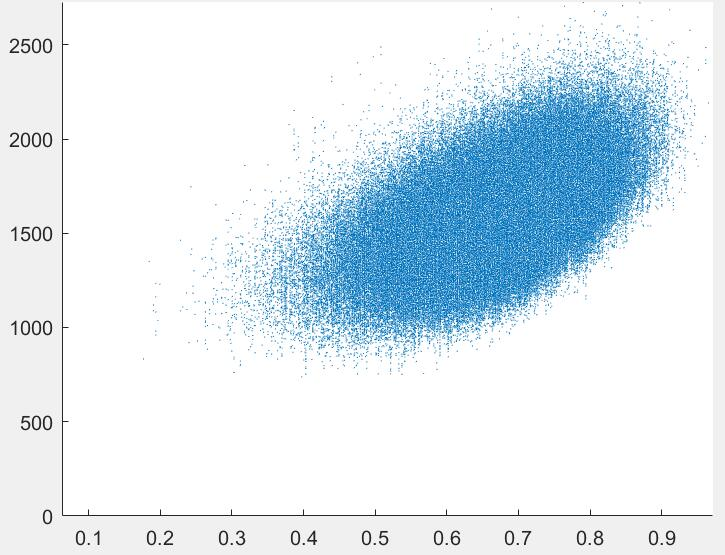
\includegraphics[scale=0.38]{400000.jpg}
            \caption{覆盖率与成本}
            \end{figure} 
        观察图像的下边缘不难发现,图像的斜率是越来越大的,
        这说明覆盖最后的百分之几的人口所需的成本很高,对运营商来说并不划算。
        为了找到$E(K)$的最大值点,我们可以把两个目标逐个击破,
        先找在同一覆盖率下所需成本最低的点,然后再在这些点之间寻找$E(K)$最大的点。
        但是由于样本空间实在太大,我们所能取得的数据仅仅是极少的情况,
        样本中的偶然性很大。为了尽可能消除这种偶然性,
        我们首先对覆盖率四舍五入至整数,如图:
        \begin{figure}[H]
            \centering
            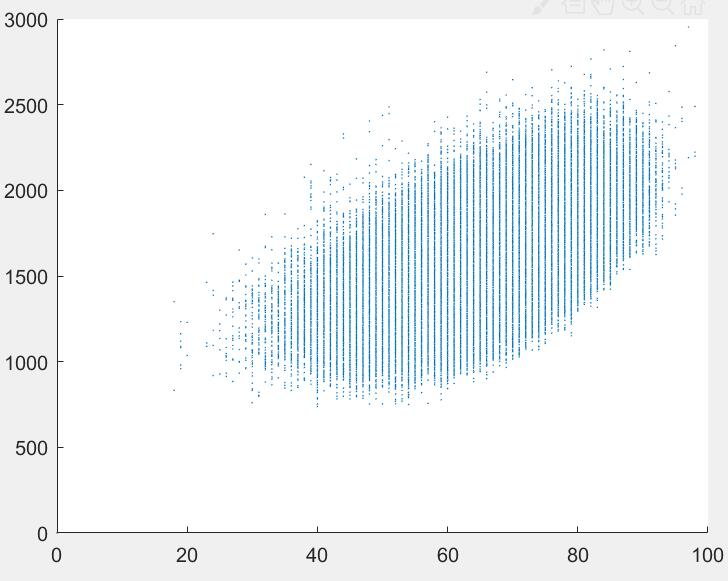
\includegraphics[scale=0.38]{400000z.jpg}
            \caption{覆盖率与成本(取整)}
            \end{figure}
        我们可以从这些数据中找到相同覆盖率下成本最低的点进行回归分析,
        得到网络覆盖率$W$关于最低成本的关系。在这里我们采用三次多项式对数据进行拟合,
        得到最低成本和覆盖率的近似方程,代入性价比函数即可求最大值。


   


\section{问题求解}

    \subsection{微波问题}

        \subsubsection{遗传算法构建}
            \begin{enumerate}
                \item 设定初始数据:
                种群大小S,繁殖代数$N$,染色体长度$l$为32,每一个碱基$k_i$有五种,
                分别代表第$i$个天线的五种相位配置方式,交叉概率$Pc$,
                变异概率$Pm$。
                \begin{large}
                    $$x = \left[ k_1 \, k_2 \, \ldots \, k_{32}\right]
                \quad (k_i =  0,1,2,3,4)$$                
                $$S = \left[x_1 \, x _2 \,  \ldots \,  x_{n}\right]^{\text{T}}$$
                
                \end{large}
                \item 计算单个个体的适应值$Ov$:\\
                不同的问题有不同的适应值计算公式,根据适应值表示该个体在整个种群中的竞争地位。
                \item 选择阶段:\\
                采用轮盘赌法,选出新的S个优势个体。
                \item 交叉阶段:\\
                采用单点交叉的交叉算子,对染色体部分碱基进行大范围交换
                \item 变异阶段:\\
                采用单点变异,对染色体单个碱基进行更改操作
                \item 重复第2步至第5步,输出最优的染色体编码,
                并将其转化为波束的矢量配置方式
            \end{enumerate}
        
        \subsubsection{微波问题1}
        使用\ref{SYDY}-波束配置方式效用评价模型做为遗传算法中第2步的适应值,
        选取的参数为:
        \begin{itemize}
            \item $a=35.5$
            \item $b=15$
            \item $c=20$
            \item $d=20$
            \item $f=10$
            \item $μ = 1$
        \end{itemize}

        得到适应度函数:
        \begin{Large}
            $$Ov = {\frac{1}{1+e^{-15·(Gv-35.5)}}}
            ×20·e^{(\frac{20-Iv}{10})}×{K}^{-1}$$
        \end{Large}
        
        运行遗传算法程序,随着迭代的次数增加,可以观察到适应度最后收敛于一稳定值:
        \begin{figure}[H]
            \centering
            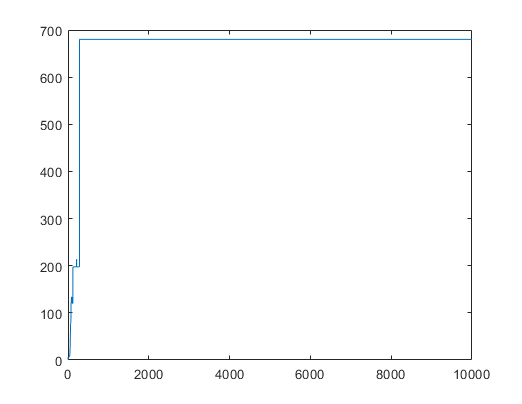
\includegraphics[scale=0.82]{lian1.png}
            \caption{微波问题1——适应度随迭代次数变化}
            \end{figure}
        得出波束最优矢量配置方式为:
              % Table generated by Excel2LaTeX from sheet 'Sheet1'
      \begin{table}[htbp]
        \centering
        \caption{微波问题1——最优配置方式}
          \begin{tabular}{cccccccccccc}
          \toprule
          天线编号   & 1      & 2      & 3      & 4      & 5      & 6      & 7      & 8      & 9      & 10     & 11 \\
          \midrule
          配置方式   & 90°    & 0°     & 180°   & 关闭     & 关闭     & 90°    & 90°    & 0°     & 270°   & 180°   & 180° \\
          \midrule
          天线编号   & 12     & 13     & 14     & 15     & 16     & 17     & 18     & 19     & 20     & 21     & 22 \\
          \midrule
          配置方式   & 0°     & 0°     & 关闭     & 180°   & 270°   & 90°    & 90°    & 270°   & 关闭     & 180°   & 90° \\
          \midrule
          天线编号   & 23     & 24     & 25     & 26     & 27     & 28     & 29     & 30     & 31     & 32     &  \\
          \midrule
          配置方式   & 180°   & 180°   & 270°   & 270°   & 90°    & 90°    & 90°    & 0°     & 180°   & 90°    &  \\
          \bottomrule
          \end{tabular}%
        \label{tab:addlabel}%
      \end{table}%

        根据波束矢量配置方式,画出合成功率的等高线图
        \begin{figure}[H]
          \centering
          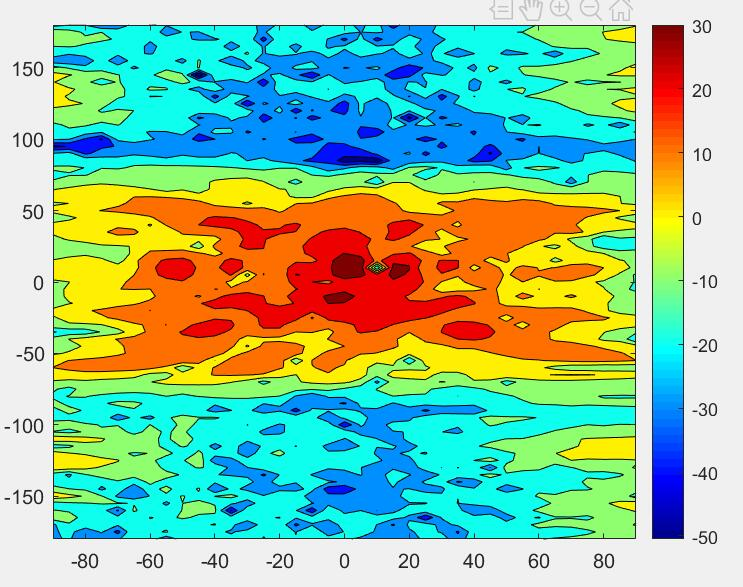
\includegraphics[scale=0.45]{h1.jpg}
          \caption{微波问题1——合成功率等高线图}
          \end{figure} 
          在该配置方式下:\begin{enumerate}
              \item AZ=10°,EL=5处,合成功率$36.05dBm $
              \item AZ=10°,EL=10处,合成功率$-19.94dBm$
              \item 旁瓣合成功率为$23dBm$
          \end{enumerate}
          


        \subsubsection{微波问题2}
        使用\ref{SYDE}-区域覆盖效用评价模型做为遗传算法中第2步的适应值,
        选取的参数为:
        \begin{itemize}
            \item $a=10$
            \item $σ = 1$
            \item $d=35.5$
            \item $f=20$
        \end{itemize}

        得到适应度函数:
        \begin{large}
            $$Ov = e^{-\frac {D}{10}}×(C+1)×\frac {1}{1+e^{-20·(M-35.5)}}$$
        \end{large}

        运行遗传算法程序,随着迭代的次数增加,可以观察到适应度收敛于一稳定值:
        \begin{figure}[H]
            \centering
            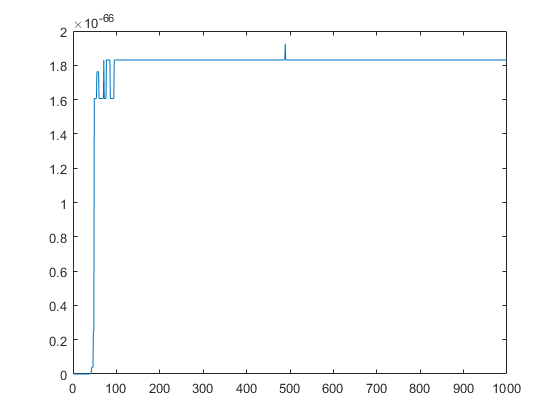
\includegraphics[scale=0.7]{lian2.png}
            \caption{微波问题2——适应度随迭代次数变化}
            \end{figure}
        选择图中的适应度最大值点,波束最优矢量配置方式为:
              % Table generated by Excel2LaTeX from sheet 'Sheet1'
      \begin{table}[htbp]
        \centering
        \caption{微波问题2——最优配置方式}
          \begin{tabular}{cccccccccccc}
          \toprule
          天线编号   & 1      & 2      & 3      & 4      & 5      & 6      & 7      & 8      & 9      & 10     & 11 \\
          \midrule
          配置方式   & 0°     & 90°    & 180°   & 180°   & 90°    & 180°   & 0°     & 270°   & 0°     & 180°   & 90° \\
          \midrule
          天线编号   & 12     & 13     & 14     & 15     & 16     & 17     & 18     & 19     & 20     & 21     & 22 \\
          \midrule
          配置方式   & 270°   & 0°     & 0°     & 0°     & 0°     & 180°   & 270°   & 90°    & 关闭     & 0°     & 180° \\
          \midrule
          天线编号   & 23     & 24     & 25     & 26     & 27     & 28     & 29     & 30     & 31     & 32     &  \\
          \midrule
          配置方式   & 0°     & 0°     & 0°     & 90°    & 0°     & 180°   & 270°   & 180°   & 0°     & 90°    &  \\
          \bottomrule
          \end{tabular}%
        \label{tab:addlabel}%
      \end{table}%

        根据波束矢量配置方式,画出合成功率的等高线图
            \begin{figure}[H]
          \centering
          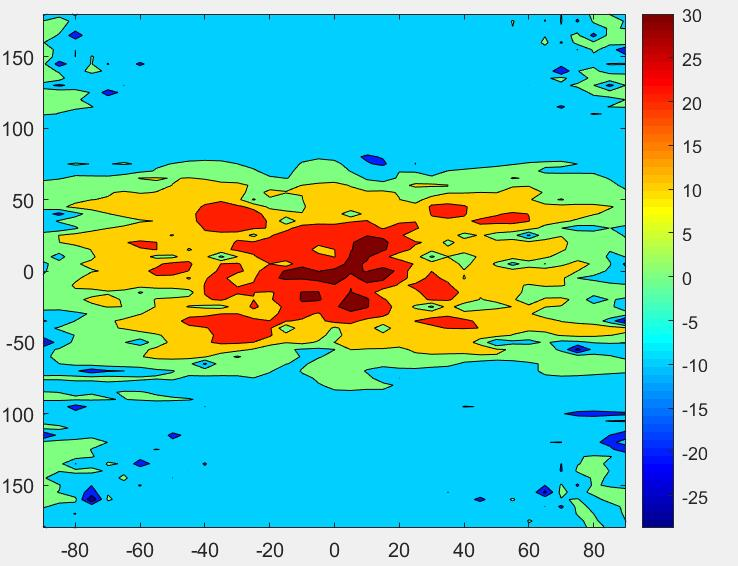
\includegraphics[scale=0.5]{h2.jpg}
          \caption{微波问题2——合成功率等高线图}
          \end{figure} 
          该配置方式下平均功率28dBm,凹坑23dBm,关闭波束1个
    


    \subsection{骨干网问题1}
        \subsubsection[网络需求评估]{各城市数据需求量评估}\label{WLXQPG}
            由文献\cite{yjJJ} 至 \cite{ysJJ},
            对2028年广东省总数据需求量进行回归分析
            \begin{gather*}
                x=[2013\,\, 2014\,\, 2015\,\, 2016\,\, 2017\,\, 2018\,\, 2019]\\
                y=[0.1\,\, 0.17\,\, 0.33\,\, 0.79\,\, 1.8\,\, 3.7\,\, 7.3]
            \end{gather*}\par
            得到回归方程$$y=0.0003915×(x-2011)^{5.512}$$\par
            代入$x=2028$,得到人均月流量$3249.33GB$。\par
            广东省人口为1.2亿,由此估计得2028年全省总数据需求量为$150.4TB/s$。\par
            对广东省各城市人口、平均年龄、人均可支配收入\upcite{CSSJ},
            根据\ref{PingFen}—城市评分模型进行评分,
            并根据\ref{ShuJv}—数据需求模型评价各个城市的需求总分(见表\ref{PF}),
            以所有城市的需求总分之和作为广东省全省的需求总分,
            并以回归分析所得的2028年全省总数据需求量为标准,
            得到单位分数对应的数据需求量,
            以此评估广东省各城市的数据需求量。
            \begin{table}[H]
                \centering
                \caption{各城市数据需求评估(数据来自\cite{CSSJ})}\label{PF}
                  \begin{tabular}{cccccccccc}
                  \toprule
                  1      & $C_k$ & $Y_k$ & $x_{k1}$ & $I_k$ & $x_{k2}$ & $P_k$ & $x_{k3}$ & $x_k$ & $N_k$ \\
                  \midrule
                  2      & 广州     & 34.4   & 100    & 5.54   & 100    & 1490.4 & 100    & 100    & 15.24 \\
                  \midrule
                  3      & 佛山     & 34.4   & 100    & 4.96   & 93.62  & 790.57 & 53.04  & 65.68  & 10.01 \\
                  \midrule
                  4      & 东莞     & 30.6   & 112.4  & 4.93   & 93.27  & 839.22 & 56.31  & 68.79  & 10.48 \\
                  \midrule
                  5      & 江门     & 34.5   & 99.71  & 2.95   & 63.31  & 459.82 & 30.85  & 43.23  & 6.588 \\
                  \midrule
                  6      & 清远     & 34.5   & 99.71  & 2.24   & 47.05  & 387.4  & 25.99  & 36.13  & 5.505 \\
                  \midrule
                  7      & 中山     & 33.5   & 102.7  & 4.69   & 90.27  & 331    & 22.21  & 43.53  & 6.634 \\
                  \midrule
                  8      & 肇庆     & 31.7   & 108.5  & 2.41   & 51.33  & 415.17 & 27.86  & 39.05  & 5.95 \\
                  \midrule
                  9      & 珠海     & 33.4   & 103    & 4.81   & 91.8   & 189.11 & 12.69  & 37.24  & 5.675 \\
                  \midrule
                  10     & 深圳     & 32.1   & 107.2  & 5.75   & 102.3  & 1302.7 & 87.4   & 92.22  & 14.05 \\
                  \midrule
                  11     & 惠州     & 31.6   & 108.9  & 3.39   & 71.4   & 483    & 32.41  & 46.82  & 7.135 \\
                  \midrule
                  12     & 云浮     & 31.2   & 110.2  & 1.92   & 38.24  & 252.69 & 16.95  & 28.56  & 4.352 \\
                  \midrule
                  13     & 韶关     & 34.7   & 99.14  & 2.37   & 50.37  & 299.76 & 20.11  & 32.73  & 4.987 \\
                  \midrule
                  14     & 河源     & 31.7   & 108.5  & 1.94   & 38.72  & 309.39 & 20.76  & 31.21  & 4.756 \\
                  \midrule
                  15     & 阳江     & 32.9   & 104.6  & 2.32   & 49.05  & 255.56 & 17.15  & 30.75  & 4.685 \\
                  \midrule
                  16     & 湛江     & 32.5   & 105.8  & 2.14   & 44.53  & 733.2  & 49.19  & 52.24  & 7.96 \\
                  \midrule
                  17     & 茂名     & 30.9   & 111.3  & 2.14   & 44.32  & 631.32 & 42.36  & 47.81  & 7.285 \\
                  \midrule
                  18     & 汕尾     & 31.3   & 109.9  & 2.1    & 43.36  & 299.36 & 20.09  & 31.89  & 4.86 \\
                  \midrule
                  19     & 揭阳     & 32     & 107.5  & 2      & 40.63  & 608.94 & 40.86  & 45.64  & 6.954 \\
                  \midrule
                  20     & 汕头     & 32.5   & 105.8  & 2.44   & 52.19  & 563.85 & 37.83  & 46.03  & 7.014 \\
                  \midrule
                  21     & 潮州     & 34.3   & 100.3  & 2.09   & 43.09  & 265.66 & 17.82  & 29.55  & 4.504 \\
                  \midrule
                  22     & 梅州     & 33.8   & 101.8  & 2.12   & 43.96  & 437.88 & 29.38  & 37.95  & 5.782 \\
                  \midrule
                         & 总和     &        & 2207   &        & 1293   &        & 761.3  & 987    & 150.4 \\
                  \bottomrule
                  \end{tabular}%
              \end{table}%

        \subsubsection[线路部署位置]{线路部署的设计}    
            \noindent 借助\ref{WLXQPG}中获取的各城市数据需求量:
            \begin{enumerate}
                \item 使用\ref{YQSFMX}:蚁群算法模型,选取的参数为
                    \begin{itemize}
                        \item $n=19$ (客观事实,其中广州市编号为1)
                        \item $a=2$
                        \item $b=1$ (蚁群算法原始权重参数)
                        \item $c=0.3$ (蚁群算法信息素挥发速度参数)
                        \item $d=0.3$ (蚂蚁走过路线时该线路增加的信息素含量)
                        \item $s=50$ (蚂蚁种群数量最终将信息素含量的大小作为边的粗细)
                    \end{itemize}
                得到:
                    \begin{figure}[H]
                      \centering
                      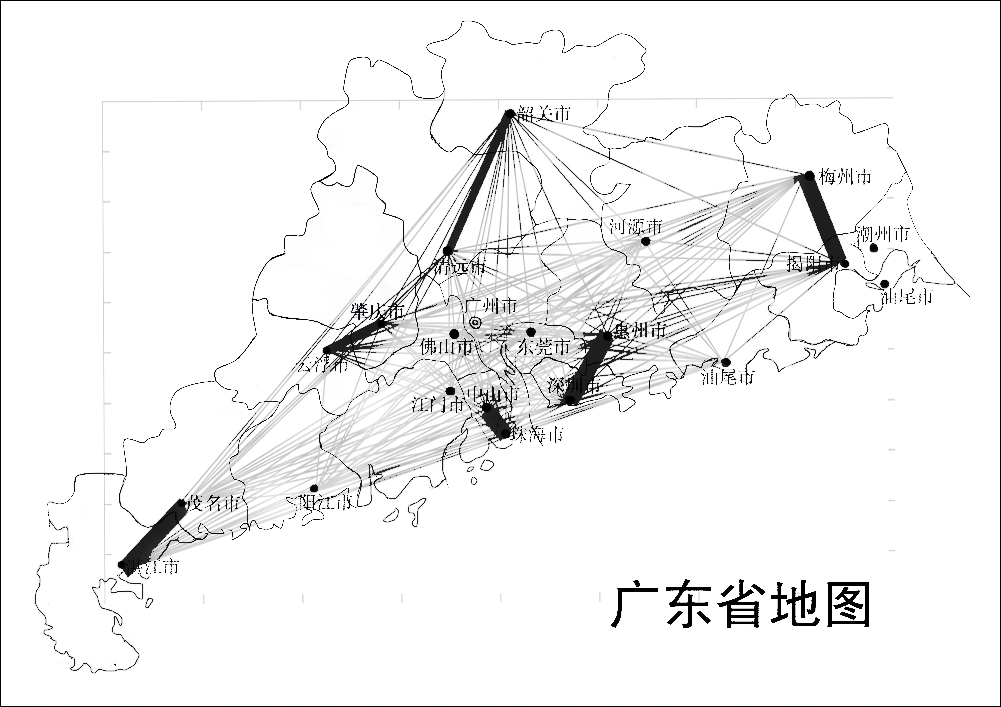
\includegraphics[scale=0.28]{YQSF.png}   %输入文件绝对路径。如果同文件夹下就不用
                      \caption{蚁群算法方案}
                      \end{figure}
                我们决定以这些边为基础创建网络。

                \item 使用\ref{ZXSCSMX}:最小生成树模型,代入的数据有:
                    \begin{itemize}
                        \item 城市距离的邻接矩阵$G_1(u,v)$:
            \begin{table}[H]
                \caption{城市距离邻接矩阵}
                \makebox[35em][c]{
                    \begin{scriptsize}
                        
                    \begin{tabular}{cccccccccccccccccccc}
                        \toprule
                        编号   & 1      & 2      & 3      & 4      & 5      & 6      & 7      & 8      & 9      & 10     & 11     & 12     & 13     & 14     & 15     & 16     & 17     & 18     & 19 \\
                        \midrule
                        1  & 0      & 19     & 50     & 62     & 64     & 74     & 80     & 98     & 106    & 115    & 128    & -1     & 162    & 196    & -1     & -1     & -1     & -1     & -1  \\
                        \midrule
                        2  & 19     & 0      & 66     & 49     & 71     & 68     & 65     & 95     & 114    & 131    & 110    & -1     & 181    & 178    & -1     & -1     & -1     & -1     & -1  \\
                        \midrule
                        3  & 50     & 66     & 0      & 86     & 98     & 76     & 130    & 90     & 67     & 66     & 176    & -1     & 124    & -1     & -1     & -1     & 167    & -1     & -1  \\
                        \midrule
                        4  & 62     & 49     & 86     & 0      & 119    & 34     & 84     & 60     & 103    & 144    & 111    & -1     & -1     & 142    & -1     & -1     & -1     & -1     & -1  \\
                        \midrule
                        5  & 64     & 71     & 98     & 119    & 0      & 137    & 84     & 162    & 164    & 153    & 134    & 129    & 168    & -1     & -1     & -1     & -1     & -1     & -1  \\
                        \midrule
                        6  & 74     & 68     & 76     & 34     & 137    & 0      & 116    & 27     & 73     & 122    & 145    & -1     & 197    & 161    & -1     & -1     & -1     & -1     & -1  \\
                        \midrule
                        7  & 80     & 65     & 130    & 84     & 84     & 116    & 0      & 143    & 176    & 195    & 51     & -1     & -1     & 152    & -1     & -1     & -1     & -1     & -1  \\
                        \midrule
                        8  & 98     & 95     & 90     & 60     & 162    & 27     & 143    & 0      & 62     & 122    & 169    & -1     & -1     & 170    & -1     & -1     & 197    & -1     & -1  \\
                        \midrule
                        9  & 106    & 114    & 67     & 103    & 164    & 73     & 176    & 62     & 0      & 65     & -1     & -1     & 150    & -1     & -1     & -1     & 136    & -1     & -1  \\
                        \midrule
                        10 & 115    & 131    & 66     & 144    & 153    & 122    & 195    & 122    & 65     & 0      & -1     & -1     & 86     & -1     & -1     & -1     & 102    & -1     & -1  \\
                        \midrule
                        11 & 128    & 110    & 176    & 111    & 134    & 145    & 51     & 169    & -1     & -1     & 0      & -1     & -1     & 119    & -1     & -1     & -1     & -1     & -1  \\
                        \midrule
                        12 & -1     & -1     & -1     & -1     & 129    & -1     & -1     & -1     & -1     & -1     & -1     & 0      & -1     & -1     & -1     & -1     & -1     & -1     & -1  \\
                        \midrule
                        13 & 162    & 181    & 124    & -1     & 168    & 197    & -1     & -1     & 150    & 86     & -1     & -1     & 0      & -1     & -1     & -1     & 124    & -1     & 148  \\
                        \midrule
                        14 & 196    & 178    & -1     & 142    & -1     & 161    & 152    & 170    & -1     & -1     & 119    & -1     & -1     & 0      & -1     & 114    & -1     & -1     & -1  \\
                        \midrule
                        15 & -1     & -1     & -1     & -1     & -1     & -1     & -1     & -1     & -1     & -1     & -1     & -1     & -1     & -1     & 0      & 76     & -1     & -1     & -1  \\
                        \midrule
                        16 & -1     & -1     & -1     & -1     & -1     & -1     & -1     & -1     & -1     & -1     & -1     & -1     & -1     & 114    & 76     & 0      & -1     & -1     & -1  \\
                        \midrule
                        17 & -1     & -1     & -1     & -1     & -1     & -1     & -1     & -1     & -1     & 102    & -1     & -1     & -1     & -1     & -1     & -1     & 0      & 131    & 173  \\
                        \midrule
                        18 & -1     & -1     & -1     & -1     & -1     & -1     & -1     & -1     & -1     & -1     & -1     & -1     & -1     & -1     & -1     & -1     & 131    & 0      & 80  \\
                        \midrule
                        19 & -1     & -1     & -1     & -1     & -1     & -1     & -1     & -1     & -1     & -1     & -1     & -1     & 148    & -1     & -1     & -1     & 173    & 80     & 0   \\
                        \bottomrule
                        \end{tabular}
                        
                    \end{scriptsize}
                }
                \end{table}

                        \item 城市需求矩阵$G_2$:
                              % Table generated by Excel2LaTeX from sheet 'Sheet1'
      \begin{table}[htbp]
        \centering
        \caption{城市需求矩阵}
          \begin{tabular}{ccccccccccc}
          \toprule
          城市     & 广州     & 佛山     & 东莞     & 江门     & 清远     & 中山     & 肇庆     & 珠海     & 深圳     & 惠州 \\
          \midrule
          需求     & 15.24  & 10.01  & 10.48  & 6.59   & 5.51   & 6.63   & 5.95   & 5.67   & 14.05  & 7.13  \\
          \midrule
          城市     & 云浮     & 韶关     & 河源     & 阳江     & 湛江     & 茂名     & 汕尾     & 潮汕     & 梅州     &  \\
          \midrule
          需求     & 4.35   & 4.99   & 4.76   & 4.69   & 7.96   & 7.28   & 4.86   & 18.47  & 5.78   &  \\
          \bottomrule
          \end{tabular}%
      \end{table}%

                        \item 城市距离与需求加权邻接矩阵$G_{0}(u',v)$:
      \begin{table}[H]
        \caption{城市距离与需求加权邻接矩阵}
        \makebox[35em][c]{
            \begin{tiny}
              
          \begin{tabular}{ccccccccccccccccccc}
          \toprule
          -1     & 8.666  & 3.380  & 2.304  & 2.125  & 1.943  & 1.739  & 1.396  & 1.815  & 1.273  & 1.004  & 0.735  & 0.809  & 0.667  & -1     & -1     & -1     & -1     & -1  \\
          \midrule
          8.666  & -1     & 2.051  & 2.237  & 1.438  & 1.600  & 1.621  & 1.086  & 1.391  & 0.859  & 0.853  & 0.507  & 0.535  & 0.543  & -1     & -1     & -1     & -1     & -1  \\
          \midrule
          3.380  & 2.051  & -1     & 1.296  & 1.070  & 1.472  & 0.832  & 1.184  & 2.387  & 1.763  & 0.553  & 0.545  & 0.806  & -1     & -1     & -1     & 0.689  & -1     & -1  \\
          \midrule
          2.304  & 2.237  & 1.296  & -1     & 0.666  & 2.561  & 0.984  & 1.351  & 1.312  & 0.627  & 0.644  & -1     & -1     & 0.520  & -1     & -1     & -1     & -1     & -1  \\
          \midrule
          2.125  & 1.438  & 1.070  & 0.666  & -1     & 0.580  & 0.892  & 0.452  & 0.783  & 0.541  & 0.483  & 0.535  & 0.401  & -1     & -1     & -1     & -1     & -1     & -1  \\
          \midrule
          1.943  & 1.600  & 1.472  & 2.561  & 0.580  & -1     & 0.711  & 2.965  & 1.869  & 0.740  & 0.497  & -1     & 0.379  & 0.460  & -1     & -1     & -1     & -1     & -1  \\
          \midrule
          1.739  & 1.621  & 0.832  & 0.984  & 0.892  & 0.711  & -1     & 0.534  & 0.748  & 0.440  & 1.316  & -1     & -1     & 0.459  & -1     & -1     & -1     & -1     & -1  \\
          \midrule
          1.396  & 1.086  & 1.184  & 1.351  & 0.452  & 2.965  & 0.534  & -1     & 2.087  & 0.692  & 0.389  & -1     & -1     & 0.400  & -1     & -1     & 0.425  & -1     & -1  \\
          \midrule
          1.815  & 1.391  & 2.387  & 1.312  & 0.783  & 1.869  & 0.748  & 2.087  & -1     & 2.146  & -1     & -1     & 0.821  & -1     & -1     & -1     & 1.020  & -1     & -1  \\
          \midrule
          1.273  & 0.859  & 1.763  & 0.627  & 0.541  & 0.740  & 0.440  & 0.692  & 2.146  & -1     & -1     & -1     & 0.908  & -1     & -1     & -1     & 0.910  & -1     & -1  \\
          \midrule
          1.004  & 0.853  & 0.553  & 0.644  & 0.483  & 0.497  & 1.316  & 0.389  & -1     & -1     & -1     & -1     & -1     & 0.499  & -1     & 0.427  & -1     & -1     & -1  \\
          \midrule
          0.735  & 0.507  & 0.545  & -1     & 0.535  & -1     & -1     & -1     & -1     & -1     & -1     & -1     & 0.405  & -1     & -1     & -1     & -1     & -1     & -1  \\
          \midrule
          0.809  & 0.535  & 0.806  & -1     & 0.401  & 0.379  & -1     & -1     & 0.821  & 0.908  & -1     & 0.405  & -1     & -1     & -1     & -1     & 0.624  & 0.815  & 0.464  \\
          \midrule
          0.667  & 0.543  & -1     & 0.520  & -1     & 0.460  & 0.459  & 0.400  & -1     & -1     & 0.499  & -1     & -1     & -1     & 0.464  & 0.691  & -1     & -1     & -1  \\
          \midrule
          -1     & -1     & -1     & -1     & -1     & -1     & -1     & -1     & -1     & -1     & -1     & -1     & -1     & 0.464  & -1     & 1.309  & -1     & -1     & -1  \\
          \midrule
          -1     & -1     & -1     & -1     & -1     & -1     & -1     & -1     & -1     & -1     & 0.427  & -1     & -1     & 0.691  & 1.309  & -1     & -1     & -1     & -1  \\
          \midrule
          -1     & -1     & 0.689  & -1     & -1     & -1     & -1     & 0.425  & 1.020  & 0.910  & -1     & -1     & 0.624  & -1     & -1     & -1     & -1     & 1.175  & 0.486  \\
          \midrule
          -1     & -1     & -1     & -1     & -1     & -1     & -1     & -1     & -1     & -1     & -1     & -1     & 0.815  & -1     & -1     & -1     & 1.175  & -1     & 1.800  \\
          \midrule
          -1     & -1     & -1     & -1     & -1     & -1     & -1     & -1     & -1     & -1     & -1     & -1     & 0.464  & -1     & -1     & -1     & 0.486  & 1.800  & -1  \\
          \bottomrule
          \end{tabular}%
        \end{tiny}
        }
      \end{table}%

                    \end{itemize}\par
                经过程序计算,得到:
                    \begin{figure}[H]
                      \centering
                      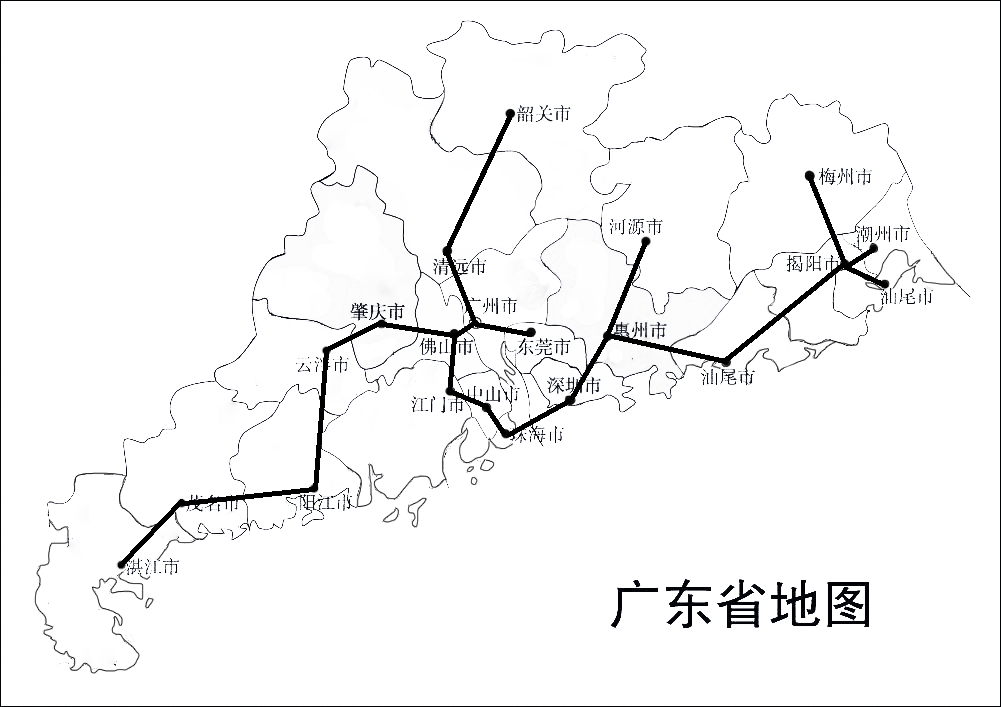
\includegraphics[scale=0.6]{ZXSCS.png}   %输入文件绝对路径。如果同文件夹下就不用
                      \caption{最小生成树方案}
                      \end{figure} 
            \end{enumerate}

            可以发现最小生成树算法得到的线路网络与蚁群算法的结果非常吻合,
            综合两个模型考虑,我们剔除了珠海到深圳横跨珠江的不符合现实的线路,
            在江门到佛山,肇庆到清远,深圳到惠州之间加入了网络线路,
            期望平衡网络流量的负载。最终确定了线路部署方案:
            \begin{figure}[H]
                \centering
                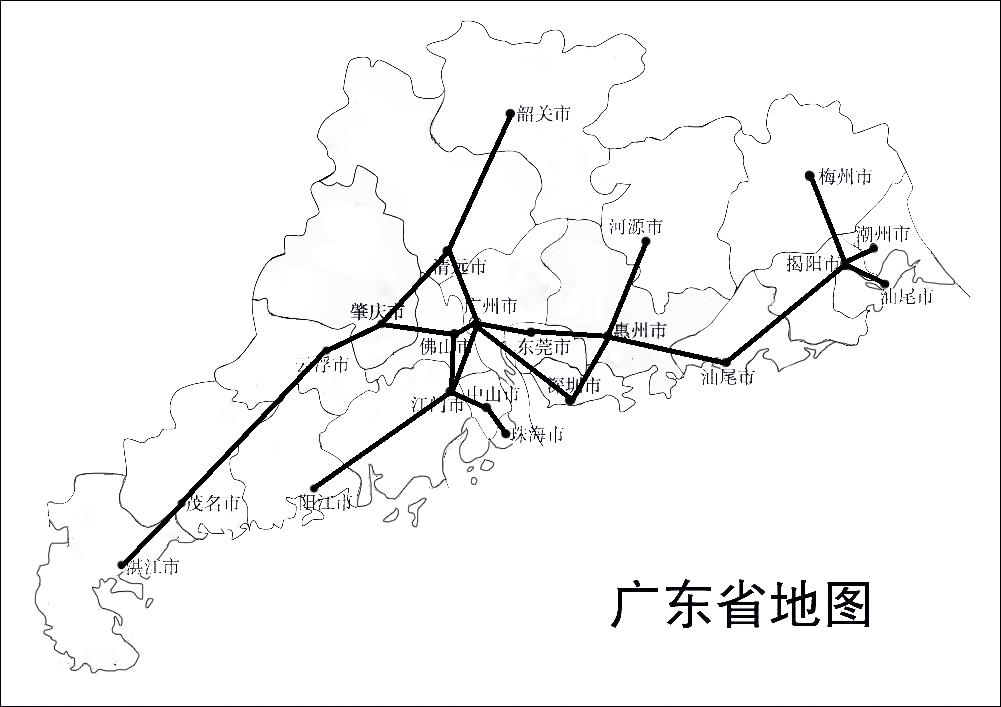
\includegraphics[scale=0.6]{over.png}   %输入文件绝对路径。如果同文件夹下就不用
                \caption{线路部署方案}
                \end{figure}

        \subsubsection{线路类型及光纤数}
            使用\ref{WLCSGS}—网络传输格式选型评价模型,其中的城市编号与路径编号为:
                  % Table generated by Excel2LaTeX from sheet 'Sheet1'
      \begin{table}[htbp]
        \centering
        \caption{城市编号}
          \begin{tabular}{cccccccc}
          \toprule
          \multicolumn{1}{c}{\textbf{1}} & \multicolumn{1}{c}{\textbf{2}} & \textbf{3} & \multicolumn{1}{c}{\textbf{4}} & \textbf{5} & \textbf{6} & \textbf{7} & \textbf{8} \\
          \midrule
          广州     & 佛山     & \multicolumn{1}{c}{东莞} & 江门     & \multicolumn{1}{c}{清远} & \multicolumn{1}{c}{中山} & \multicolumn{1}{c}{肇庆} & \multicolumn{1}{c}{珠海} \\
          \midrule
          \multicolumn{1}{c}{\textbf{9}} & \multicolumn{1}{c}{\textbf{10}} & \textbf{11} & \multicolumn{1}{c}{\textbf{12}} & \textbf{13} & \textbf{14} & \textbf{15} & \textbf{16} \\
          \midrule
          深圳     & 惠州     & \multicolumn{1}{c}{云浮} & 韶关     & \multicolumn{1}{c}{河源} & \multicolumn{1}{c}{阳江} & \multicolumn{1}{c}{湛江} & \multicolumn{1}{c}{茂名} \\
          \midrule
          \multicolumn{1}{c}{\textbf{17}} & \multicolumn{2}{c}{\textbf{18}} & \multicolumn{1}{c}{\textbf{19}} &        &        &        &  \\
          \midrule
          汕尾     & \multicolumn{2}{c}{潮汕三市} & 梅州     &        &        &        &  \\
          \bottomrule
          \end{tabular}%
      \end{table}%

      \begin{table}[htbp]
        \centering
        \caption{路径编号}
        \begin{footnotesize}
            
          \begin{tabular}{cccccccc}
          \toprule
          \textbf{编号} & \textbf{1} & \textbf{2} & \textbf{3} & \textbf{4} & \textbf{5} & \textbf{6} & \textbf{7} \\
          \midrule
          端点     & 广州 & 广州 & 广州 & 佛山 & 广州 & 江门 & 佛山 \\
          \midrule
          端点     & 佛山 & 东莞 & 江门 & 江门 & 清远 & 中山 & 肇庆 \\
          \midrule
          距离     & 19.1   & 49.9   & 62.2   & 48.7   & 64     & 33.9   & 64.6 \\
          \midrule
          \textbf{编号} & \textbf{8} & \textbf{9} & \textbf{10} & \textbf{11} & \textbf{12} & \textbf{13} & \textbf{14} \\
          \midrule
          端点     & 肇庆 & 中山 & 广州 & 惠州 & 惠州 & 肇庆 & 清远 \\
          \midrule
          端点     & 清远 & 珠海 & 深圳 & 东莞 & 深圳 & 云浮 & 韶关 \\
          \midrule
          距离     & 84.3   & 27.4   & 106    & 65.6   & 64.8   & 51.4   & 128.7 \\
          \midrule
          \textbf{编号} & \textbf{15} & \textbf{16} & \textbf{17} & \textbf{18} & \textbf{19} & \textbf{20} & \textbf{21} \\
          \midrule
          端点     & 惠州 & 江门 & 云浮 & 湛江 & 惠州 & 汕尾 & 揭阳 \\
          \midrule
          端点     & 河源 & 阳江 & 茂名 & 茂名 & 汕尾 & 揭阳 & 梅州 \\
          \midrule
          距离     & 85.9   & 142.1  & 179    & 76.4   & 102    & 130.5  & 80.6 \\
          \bottomrule
          \end{tabular}%
        \end{footnotesize}
      \end{table}%
         由此可以得到网络传输格式设置向量。运行遗传算法程序,  
     采用的新适应度函数保留了大部分条件十分接近目标的值,如图
     \begin{figure}[H]
        \centering
        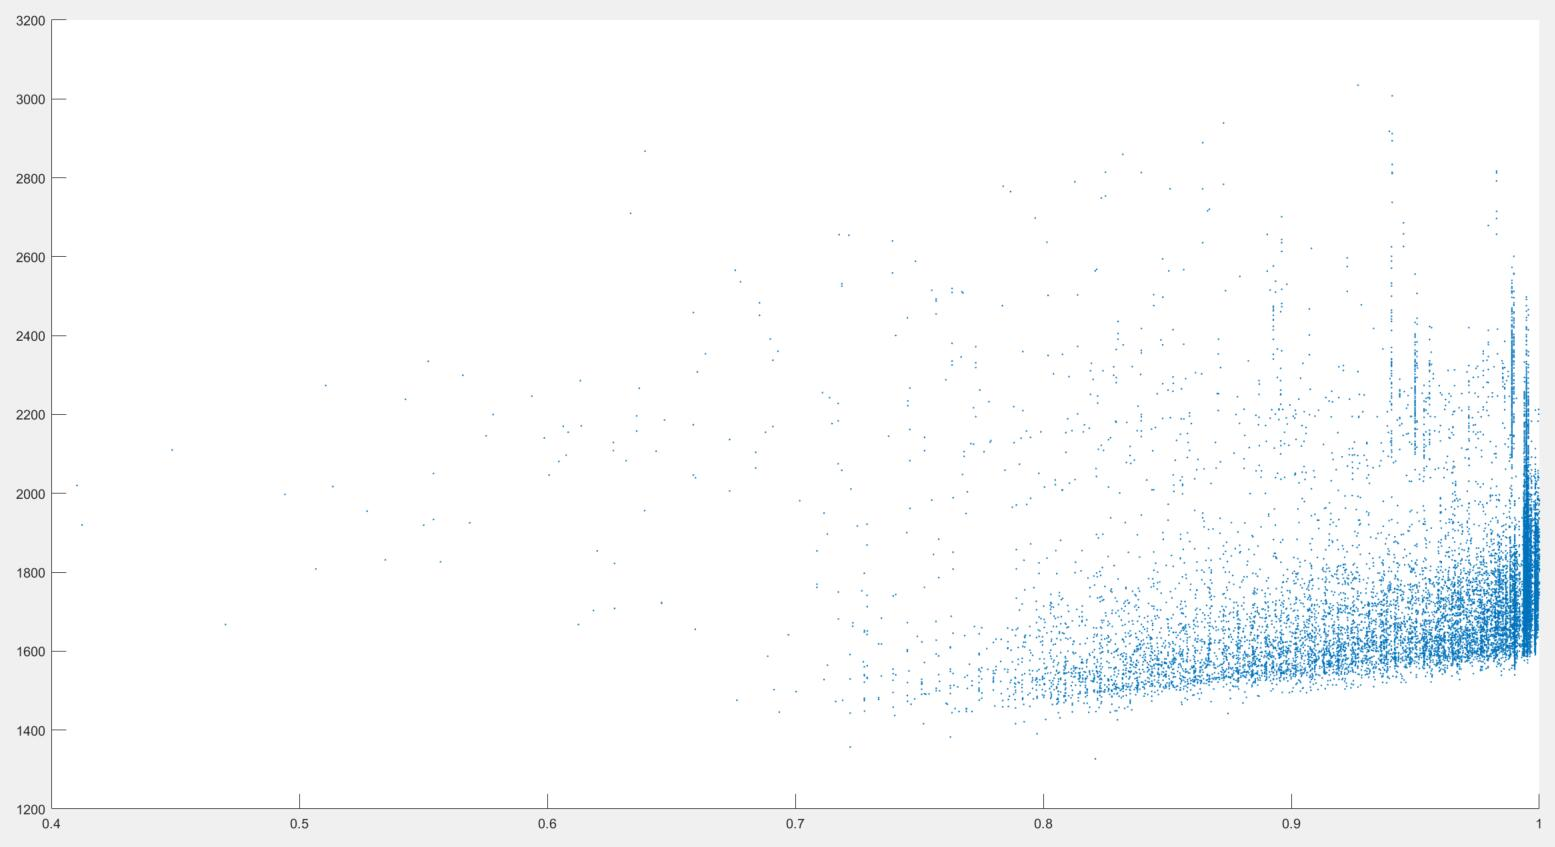
\includegraphics[scale=0.8]{cos.jpg}
        \caption{覆盖率与成本}
        \end{figure} 
     我们选取其中最优值点$K_m$,观察这个配置方式经过最大流算法计算后的残余网络发现,
     网路的流量没有从路径12和路径4走,于是我们改进了由网络构建模型的到了网络构建图,
     删除了这两条路径。继续观察残余网络发现网络的配置仍然有冗余,
     在减少冗余配置之后,得到有着最低成本$Cost_{min}=1439.5X$的最优结果
           % Table generated by Excel2LaTeX from sheet 'Sheet1'
           \begin{table}[htbp]
            \centering
            \caption{骨干网问题1——最终网络部署方案}
              \begin{scriptsize}
                  
              \begin{tabular}{cccccccccccc}
              \toprule
              线路编号   & 1      & 2      & 3      & 4      & 5      & 6      & 7      & 8      & 9      & 10     & 11 \\
              \midrule
              线路容量GB/s & 36000  & 52800  & 24800  & 0      & 12000  & 12800  & 25600  & 1200   & 6400   & 14400  & 42400 \\
              \midrule
              线路编号   & 12     & 13     & 14     & 15     & 16     & 17     & 18     & 19     & 20     & 21     &  \\
              \midrule
              线路容量GB/s & 0      & 20800  & 5200   & 5400   & 4800   & 16000  & 8800   & 30000  & 25200  & 6000   &  \\
              \bottomrule
              \end{tabular}
            \end{scriptsize}
          \end{table}%
    
            即:\par
            \begin{figure}[H]
                \centering
                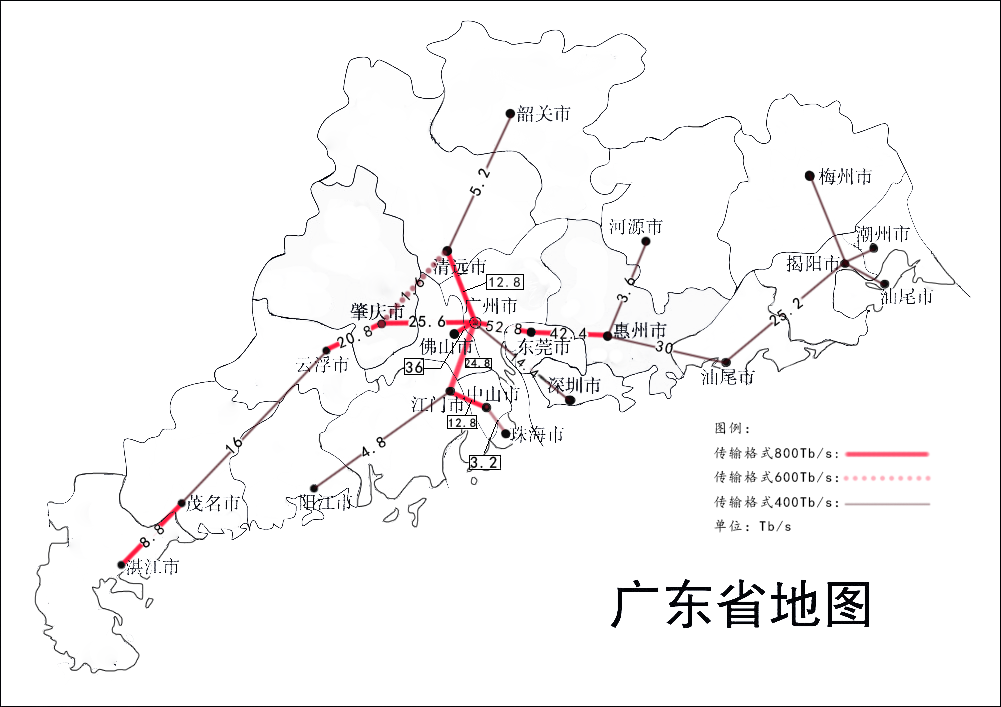
\includegraphics[scale=0.4]{overG1.png}   %输入文件绝对路径。如果同文件夹下就不用
                \caption{骨干网问题1——最终网络部署方案}
                \end{figure} 


    \subsection{骨干网问题2}
        如\ref{WLCSXJB}—网络传输性价比模型所说,对数据进行回归分析:
        \begin{figure}[H]
            \centering
            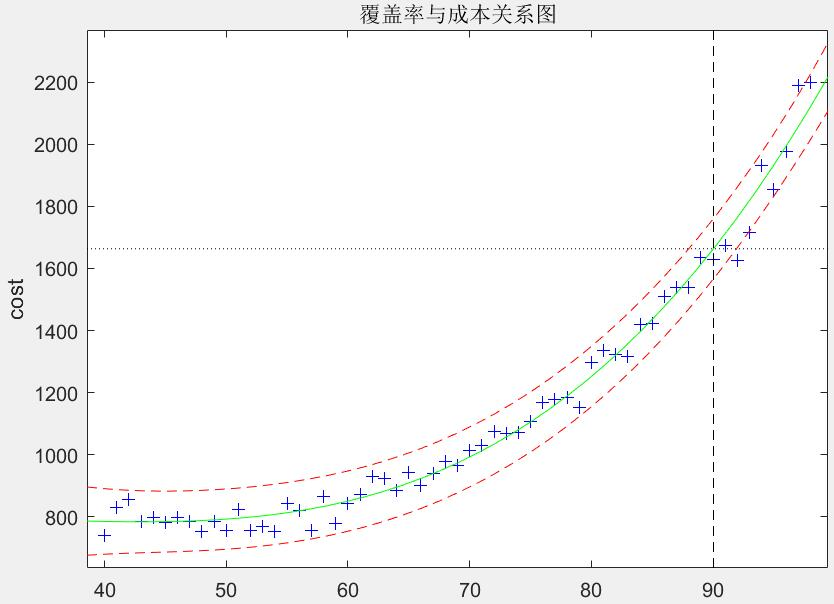
\includegraphics[scale=0.6]{cosHG.jpg}   %输入文件绝对路径。如果同文件夹下就不用
            \caption{覆盖率与成本关系图}
            \end{figure} 
        得到三次拟合方程
        $$Cost_{min}=0.0046W^3-0.5804W^2+19.08888W+594.1596$$\par
        则
        $$E(K)=\frac{W}{Cost_{min}}=\frac{1}{0.0046W^2-0.5804W+19.08888+\frac{594.1596}{W}}$$\par
        $E(k)$的图像为:
        \begin{figure}[H]
            \centering
            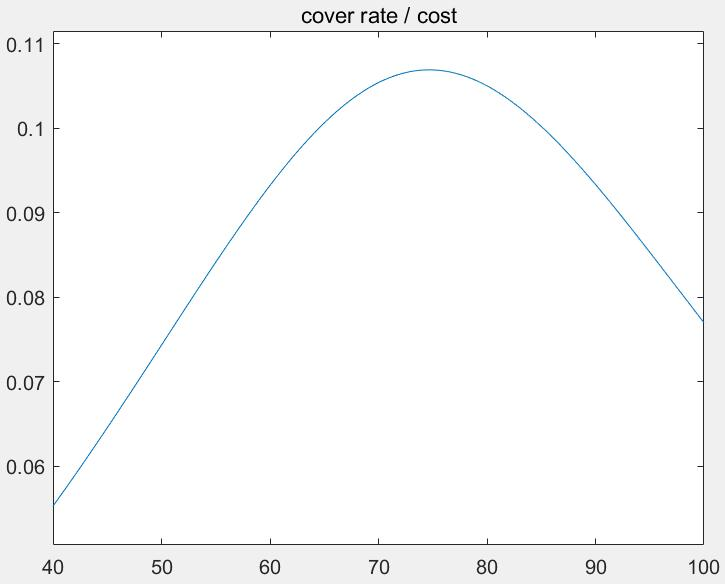
\includegraphics[scale=0.6]{cosEK.jpg}   %输入文件绝对路径。如果同文件夹下就不用
            \caption{$E(k)$}
            \end{figure} 
        取得最大点时候 $W=75~~E(K)=0.1069$,网络部署方案为
              % Table generated by Excel2LaTeX from sheet 'Sheet1'
      \begin{table}[htbp]
        \centering
        \caption{骨干网问题2——最终网络部署方案}
        \begin{scriptsize}
          \begin{tabular}{cccccccccccc}
          \toprule
          线路编号   & 1      & 2      & 3      & 4      & 5      & 6      & 7      & 8      & 9      & 10     & 11 \\
          \midrule
          线路容量Gb/s & 19200  & 16000  & 24000  & 1600   & 16000  & 17600  & 11200  & 16800  & 4000   & 31200  & 15200 \\
          \midrule
          线路编号   & 12     & 13     & 14     & 15     & 16     & 17     & 18     & 19     & 20     & 21     &  \\
          \midrule
          线路容量Gb/s & 13600  & 24800  & 800    & 4800   & 6000   & 12800  & 7200   & 19600  & 2000   & 3600   &  \\
          \bottomrule
          \end{tabular}%
        \end{scriptsize}
      \end{table}%

        该种网络选型方式下网络的性价比最高
\newpage
\section{模型的评价}
    \subsection{模型的优点}
        \begin{enumerate}
            \item 微波问题和骨干网问题都运用了遗传算法,遗传算法正适合解决这样搜索空间非常庞大的问题。
            \item 骨干网络的构建采用多种方法结合考虑,使结果更可靠。
        \end{enumerate}
    \subsection{模型的缺点}
        \begin{enumerate}
            \item 遗传算法的交叉步骤,采用的是单点交叉,所以在遗传的过程中有可能会丢失当前的优势碱基序列。
            \item 波束配置方式效用评价模型和区域覆盖效用评价模型的构建还不理想导致遗传算法的收敛速度不够快,得出结果的好坏也不稳定。
            \item 进行数据回归分析时,选取的拟合函数具有一定的主观性。
            \item 在运用层次分析法进行城市需求量评估时候,评估的尺度存在一定的主观性。
            \item 网络流模型中,我们选择先构建网络再选择线路的容量,没有对两个方法的综合考虑。
            \item 采用多种方式结合建模时,没有仔细考虑两种方式对应的权重,主观性较大。
        \end{enumerate}
    \subsection{模型的推广}
        \begin{enumerate}
            \item 微波问题中模型不仅适用于有32个波束的相控阵天线,对有任意个波束的相控阵天线或相控阵雷达以及其他阵列信号的处理仍然适用
            \item 骨干网问题中的模型不仅仅适用于广东省骨干网络建设,对于其他省份的骨干网络以及城市之内的地区网等中小规模的网络建设也具有指导意义。
        \end{enumerate}

\section{模型的改进}
    \begin{enumerate}
        \item 针对遗传算法中优良个体容易被变异破坏的问题,可以动态选择遗传概率,在只有极少数优良个体时候应该防止优良个体变异,而当整个种群集体差异度较小时候可以选择较高的变异机率使防止种群在局部最优解中停滞。
        \item 微波问题中我们选取单个方向代替正负2.5度的空间范围,这个估计比较粗糙,可以采用适当的插值法填补空隙,使得模型的精度更高。
        \item 在骨干网问题中同时考虑如何构建网络和选择线路的格式和容量,更加整体的考虑广东省骨干网的规划。
    \end{enumerate}
\newpage
\begin{thebibliography}{20}   %表示参考文献最大数量
    %每个bibitem表示一份文献
    %第一个参数这里没用(不显示),用于交叉引用
    %第二个参数就是显示的内容
    \bibitem{CSSJ}{广东省统计局,广东统计信息网(及首页中各市链接), \\
        http://stats.gd.gov.cn/, 2019.5.12.}
    \bibitem{yjJJ}{中华人民共和国工业和信息化部,2019年1-4月份通信业经济运行情况,\\
        http://www.miit.gov.cn/n1146285/n1146352/n3054355/n3057511/\\
        n3057518/c6969297/content.html, 2019.5.31}
    \bibitem{yqJJ}{中华人民共和国工业和信息化部,2017年1-4月份通信业经济运行情况,\\
        http://www.miit.gov.cn/n1146312/n1146904/n1648372/c5653421/\\
        content.html, 2019.5.31}
    \bibitem{ylJJ}{中华人民共和国工业和信息化部,2016年8月份通信业经济运行情况,\\
        http://www.miit.gov.cn/n1146285/n1146352/n3054355/n3057511/\\
        n3057518/c5264001/content.html, 2019.5.31}
    \bibitem{ywJJ}{中华人民共和国工业和信息化部,2015年7月份通信业经济运行情况,\\
        http://www.miit.gov.cn/n1146285/n1146352/n3054355/n3057511/\\
        n3057518/c3602990/content.html, 2019.5.31}
    \bibitem{ysJJ}{中华人民共和国工业和信息化部,2014年6月份通信业经济运行情况,\\
        http://www.miit.gov.cn/n1146312/n1146904/n1648372/c3336719/\\
        content.html, 2019.5.31}
    \bibitem{}{Gallager R G, Humblet P A, Spira P M. A distributed 
        algorithm for minimum-weight spanning trees[J]. 
        ACM Transactions on Programming Languages and systems 
        (TOPLAS), 1983, 5(1): 66-77.}
    \bibitem{}{Davis L. Handbook of genetic algorithms[J]. 1991.}
    \bibitem{}{曾建军、李世航、王永国、叶仁玉、MATLAB语言与数学建模,安徽:安徽大学出版社,2005.}
    \bibitem{}{房少梅,数学建模理论、方法及应用,北京:科学出版社,2014.}
    
    %文献按正文中的引用次序列出,其中书籍的表述方式为:
    %[编号] 作者,书名,出版地:出版社,出版年。
    %参考文献中期刊杂志论文的表述方式为:
    %[编号] 作者,论文名,杂志名,卷期号:起止页码,出版年。
    %参考文献中网上资源的表述方式为:
    %[编号] 作者,资源标题,网址,访问时间(年月日)。
\end{thebibliography}
\begin{appendices}
    \section{遗传算法模型——微波问题一 Matlab代码}

    \begin{scriptsize}
    \begin{lstlisting}[language=Matlab]
    function main()
init();
process=zeros(1,50000);%统计遗传算法的进步过程
x=(1:50000);
generation=10000;
popsize = 100;  %种群大小
chromlenth = 32;    %染色体长度
pc = 0.7;   %交叉概率
pm = 0.3;  %变异概率
pop = initpop(popsize, chromlenth);  %染色体处理
for i = 1:generation
    if(mod(i,500)==0)
    fp=fopen([strrep(datestr(datetime),':','-'),'.txt'],'a');
    fprintf(fp,'i=%d \n',i);
    for k = 1:100
        fprintf(fp,'%d ',pop(k,:));
        fprintf(fp,'\n');
        fprintf(fp,'%d ',objvalue(k));
        fprintf(fp,'\n');
    end
    fclose(fp)
end
    %计算适应度值(函数值)
    objvalue = cal_objvalue(pop);
    fitvalue = objvalue;
    %选择操作
    newpop = selection(pop,fitvalue);
    %交叉操作
    newpop = crossover(newpop,pc);
    %变异操作
    newpop = mutation(newpop,pm);
    %更新种群
    pop = newpop;
    %寻找最优解
    [bestindividual,bestfit] = best(pop,fitvalue);
    process(i)=bestfit;
    display(bestfit);
    display(i);
    figure(3);
    plot(x(1:i),process(1:i))
end
    serve = bestindividual;
    figure(4);
    surfdisplay(serve); %生成最优排列的图像
    save txt serve;
    display(serve);
end

function init()
    clear;
    clc;
    clc;
    clear;  %清空所有操作
    load raw_data
    global Mag
    global Mag_pow10
    global Phase_raw 
    global Phase
    global Phase_cos
    global Phase_sin
   
   Mag = raw_data.LogMag;
   Mag(find(isnan(Mag))) = -10;
   Mag(find(isinf(Mag))) = -10;
   Mag_pow10= (10.^(Mag/20));
   Phase_raw = raw_data.Phase;
   Phase_raw(find(isnan(Phase_raw))) = 0;
   Phase_raw(find(isinf(Phase_raw))) = 0;
   Phase=Phase_raw/180*pi;
   Phase(find(isnan(Phase))) = 0;
   Phase(find(isinf(Phase))) = 0;
   Phase_cos=cos(Phase);
   Phase_sin=sin(Phase);  
   %LogMag和Phase数据处理,将inf和nan全部变成0;
   
function pop = initpop(popsize, chromlenth)
pop = round(4*rand(popsize, chromlenth));    %染色体处理
%染色体一共有五种碱基,
%其中0~4代表着关闭/打开0°/打开90°/打开180°/打开270°
end

function objvalue = cal_objvalue(pop)
global Phase_cos
global Phase_sin
global Mag_pow10
interference_AZ=10;%干扰点俯仰角下边
interference_EL=10;%干扰点水平角下标
goal_AZ=10;%目标点俯仰角下标
goal_EL=5;%目标点水平角
goal_index_AZ=(goal_AZ+180)/5+1;%目标点水平角的下标=39
goal_index_EL=(goal_EL+90)/5+1;%目标点俯仰角角的下标=20
interference_index_AZ=(interference_AZ+180) / 5 + 1;
%干扰点水平角下标=39
interference_index_EL=(interference_EL+90 ) / 5 + 1;
%干扰点俯仰角下标=21
for j = 1 : 100
goal_component_cos = 0; %初始化目标值,干扰值
goal_component_sin = 0;%
interference_component_cos = 0;
interference_component_sin= 0;
goal_value = 0;
interference_value = 0;

    for i = 1 : 32
        if(pop(j,i) == 0) %假如遇到有关闭的情况就直接跳过
            continue;
        end
    
    k = pop(j,i);   %取出当前的配置方式

    LinM=Mag_pow10(goal_index_AZ,goal_index_EL,i,k);
    LinP=Phase_cos(goal_index_AZ,goal_index_EL,i,k);
    goal_component_cos = goal_component_cos + LinM.*LinM;

    LinM=Mag_pow10(goal_index_AZ,goal_index_EL,i,k);
    LinP=Phase_sin(goal_index_AZ,goal_index_EL,i,k);
    goal_component_sin = goal_component_sin + LinM.*LinP;

    LinM=Mag_pow10(interference_index_AZ,interference_index_EL,i,k);
    LinP=Phase_cos(interference_index_AZ,interference_index_EL,i,k);
    interference_component_cos = interference_component_cos + LinM.*LinP;

    LinM=Mag_pow10(interference_index_AZ,interference_index_EL,i,k);
    LinP=Phase_sin(interference_index_AZ,interference_index_EL,i,k);
    interference_component_sin = interference_component_sin + LinM.*LinP;
    end

    goal_value = (goal_component_cos.^2 + goal_component_sin.^2).^(1/2);

    Linc=interference_component_cos;
    Lins=interference_component_sin;
    interference_value = ( Linc.^2 + Lins.^2 ).^(1/2);
    
    goal_value = 20 * (log10(goal_value));
    display(interference_value);
    interference_value = 20 * (log10(interference_value)); 
    %按照dbm和信号幅度的运算公式以及矢量的正交相加减最后求其长度
    display(interference_value);
    display(goal_value);
%分配权重(重点考虑!!适应度函数很重要,因为这道题有两个变量,
%如何配置两者的权重就很关键)
%首先目标波束一定要为35以上,不然其贡献度瞬间下降,用标记统一化实现

    %权重:50/20;
    SIGMOID=1/(1+exp((-(goal_value-35.5)*15)));
    objvalue(1,j) = SIGMOID*20*exp((20-interference_value)/10);
    %对于特定的第一问的两个位置进行计算;

end

%关于编译
%函数说明
%输入变量:pop:五进制种群,pm:变异概率
%输出变量:newpop变异以后的种群
function [newpop] = mutation(pop,pm)
[px,py] = size(pop);    %同selection
newpop = ones(size(pop));%初始化
for i = 1:px
    if(rand<pm) %触发变异概率
        mpoint = round(rand*py);    %随机选取变异的碱基位置
       if mpoint <= 0;  %鲁棒性
            mpoint = 1;
        end
        newpop(i,:) = pop(i,:);
        %新加入变异
        k = newpop(i,mpoint);   %保存原先的位置碱基种类
        while(k == newpop(i,mpoint))    
        %一直更新直到出现和原先位置碱基种类不一样的情况
            k = round(4*rand(1));
        end
        newpop(i,mpoint) = k;   %更新当前位置碱基种类
    else newpop(i,:) = pop(i,:); %反之不突变
    end
end

%如何选择新的个体
%输入变量:pop五进制种群,fitvalue:适应度值
%输出变量:newpop选择以后的五进制种群
function [newpop] = selection(pop,fitvalue)
%构造轮盘
[px,py] = size(pop);    %px是种群大小,py是染色体长度
totalfit = sum(fitvalue);   %求和所有目标函数
p_fitvalue = fitvalue/totalfit; 
%求出每一个个体求出其在整个种群中的比重
p_fitvalue = cumsum(p_fitvalue);%概率前缀和排序
ms = sort(rand(px,1));%随机选取100个概率数并从小到大排列
fitin = 1;  %初始化筛选
newin = 1;
while newin<=px
    if(ms(newin)) < p_fitvalue(fitin) 
    %当随机选取的概率数小于当前的个体比重,即个体占优势,繁殖
        newpop(newin,:)=pop(fitin,:); 
        newin = newin+1;
    else
        fitin=fitin+1; %反之阉割
    end
end

%求最优适应度函数
%输入变量:pop:种群,fitvalue:种群适应度
%输出变量:bestindividual:最佳个体,bestfit:最佳适应度值
function [bestindividual, bestfit] = best(pop,fitvalue)
[px,py] = size(pop);
bestindividual = pop(1,:);
bestfit = fitvalue(1);
for i = 2:px
    if fitvalue(i)>bestfit  %就是找最大值,没什么好说的
        bestindividual = pop(i,:);
        bestfit = fitvalue(i);
    end
end

%交叉变换
%输入变量:pop:五进制的父代种群数,pc:交叉的概率
%输出变量:newpop:交叉后的种群数
function [newpop] = crossover(pop,pc)
[px,py] = size(pop);    %同selection
newpop = ones(size(pop));
for i = 1:2:px-1    %每相邻两个个体就选取
    if(rand<pc) %触发交叉概率
        cpoint = round(rand*py);    
        %标记交叉互换碱基的位置
        newpop(i,:) = [pop(i,1:cpoint),pop(i+1,cpoint+1:py)]; 
        %将后面全部换掉
        newpop(i+1,:) = [pop(i+1,1:cpoint),pop(i,cpoint+1:py)];
    else
        newpop(i,:) = pop(i,:); %否则继续繁殖
        newpop(i+1,:) = pop(i+1,:);
    end
end

function surfdisplay(serve) %用来打印最优解的三维图
load raw_data
global Phase_cos
global Phase_sin
global Mag_pow10
y1 = raw_data.AZ(:,1);
x1 = raw_data.EL(1,:);
x = zeros(73, 37);
y = zeros(73, 37);
for i = 1 : 32
    if(serve(i) == 0) 
        continue;
    end
x = x + Mag_pow10(:,:,i,serve(i)).*Phase_cos(:,:,i,serve(i));
y = y + Mag_pow10(:,:,i,serve(i)).*Phase_sin(:,:,i,serve(i));
end
field_ans = (x.^2 + y.^2).^(1/2);
field_ans = 20 * (log10(field_ans));    
%对于每一个特定的染色体,生成整个图像的值;
surf(x1, y1, field_ans);

        \end{lstlisting}
    \end{scriptsize}

    \section{遗传算法模型——微波问题二 Matlab代码}

    \begin{scriptsize}
        \begin{lstlisting}[language=Matlab]
    function main()
    init();
    process=zeros(1,50000);%统计遗传算法的进步过程
    x=(1:50000);
    generation=1000;
    popsize = 100;  %种群大小
    chromlenth = 32;    %染色体长度
    pc = 0.7;   %交叉概率
    pm = 0.15;  %变异概率
    pop = initpop(popsize, chromlenth);  %染色体处理
    for i = 1:generation
        objvalue = cal_objvalue(pop);
        fitvalue = objvalue;
        %选择操作
        newpop = selection(pop,fitvalue);
        %交叉操作
        newpop = crossover(newpop,pc);
        %变异操作
        newpop = mutation(newpop,pm);
        %更新种群
        pop = newpop;
        %寻找最优解
        [bestindividual,bestfit] = best(pop,fitvalue);
        process(i)=bestfit;
        display(bestfit);
        display(i);
        figure(3);
        plot(x(1:i),process(1:i))
    end
        serve = bestindividual;
        save txt serve;
        display(serve);
    
    function objvalue = cal_objvalue(pop)
    global Phase_cos
    global Phase_sin
    global Mag_pow10
    range_AZ_min_index=(-30+180)/5+1;%范围水平角最小边界
    range_AZ_max_index= (30+180)/5+1;%范围水平角最大边界
    range_EL_min_index=(-15+90)/5+1;%范围俯仰角最小边界
    range_EL_max_index= (15+90)/5+1;%范围俯仰角最大边界
    for j = 1 : 100
    mix_field_average=0;
    mix_field_cos=zeros(360/5+1,180/5+1);
    mix_field_sin=zeros(360/5+1,180/5+1);
    mix_field_value=zeros(360/5+1,180/5+1);
    mix_field_max=-50;
    mix_field_min=99999;
        for i = 1 : 32
            close_count=0;
            if(pop(j,i) == 0) %假如遇到有关闭的情况就直接跳过
                close_count=close_count+1;
                continue;
            end
        
           k = pop(j,i);   

        LinM=Mag_pow10(:,:,i,k);
        Linc=Phase_cos(:,:,i,k);
        Lins=Phase_sin(:,:,i,k);
        mix_field_cos = mix_field_cos + LinM.*Linc;%矢量叠加横轴
        mix_field_sin = mix_field_sin + LinM.*Lins;%矢量叠加纵轴

        end
        mix_field_value = (mix_field_cos.^2 + mix_field_sin.^2).^(1/2);
        %是强度值不是dbm单位
        for az = range_AZ_min_index:range_AZ_max_index
            for el = range_EL_min_index:range_EL_max_index
                if  mix_field_value(az,el)>mix_field_max
                    mix_field_max=mix_field_value(az,el);
                end
                if mix_field_value(az,el)<mix_field_min
                    mix_field_min=mix_field_value(az,el);
                end
                mix_field_average = mix_field_average + mix_field_value(az,el);
            end
        end

        LinAZMA=range_AZ_max_index;
        LinAZMi=range_AZ_min_index;
        LinELMA=range_EL_max_index;
        LinELMi=range_EL_min_index;
        LinAR=mix_field_average;
        mix_field_average=LinAR/((LinAZMA-LinAZMi)+1)/((LinELMA-LinELMi)+1);
        %mix_field_average=20 * (log10(mix_field_average));%强度值转换为dbm单位
        mix_field_average=20 *(log10(mix_field_average));
        mix_field_diff=20*(log10(mix_field_max)-log10(mix_field_min))
        %display(mix_field_average);
        %display(i)
        display(mix_field_average)
         %按照dbm和信号幅度的运算公式以及矢量的正交相加减最后求其长度
        
        Dw=1/exp(mix_field_diff/10);
        Cw=(close_count+1);
        Mw=1/(1+exp(-(mix_field_average-35.5)*20));
        objvalue(1,j) = Dw*Cw*Mw;
    
    end
    
    function init()
        clear;
        clc;
        clc;
        clear;  %清空所有操作
        load raw_data
        global Mag
        global Mag_pow10
        global Phase_raw 
        global Phase
        global Phase_cos
        global Phase_sin
       
       Mag = raw_data.LogMag;
       Mag(find(isnan(Mag))) = -10;
       Mag(find(isinf(Mag))) = -10;
       Mag_pow10= (10.^(Mag/20));
       %Mag_pow10= (10.^(Mag/20));
       Phase_raw = raw_data.Phase;
       Phase_raw(find(isnan(Phase_raw))) = 0;
       Phase_raw(find(isinf(Phase_raw))) = 0;
       Phase=Phase_raw/180*pi;
       Phase(find(isnan(Phase))) = 0;
       Phase(find(isinf(Phase))) = 0;
       Phase_cos=cos(Phase);
       Phase_sin=sin(Phase);  %LogMag和Phase数据处理,将inf和nan全部变成0;
       
    function pop = initpop(popsize, chromlenth)
    pop = round(4*rand(popsize, chromlenth));    %染色体处理
    %染色体一共有五种碱基,0~4代表着关闭/打开0°/打开90°/打开180°/打开270°
    end               
       
    %关于编译
    %函数说明
    %输入变量:pop:五进制种群,pm:变异概率
    %输出变量:newpop变异以后的种群
    function [newpop] = mutation(pop,pm)
    [px,py] = size(pop);    %同selection
    newpop = ones(size(pop));%初始化
    for i = 1:px
        if(rand<pm) %触发变异概率
            mpoint = round(rand*py);    %随机选取变异的碱基位置
           if mpoint <= 0;  %鲁棒性
                mpoint = 1;
            end
            newpop(i,:) = pop(i,:);
            %新加入变异
            k = newpop(i,mpoint);   %保存原先的位置碱基种类
            while(k == newpop(i,mpoint))    
            %一直更新直到出现和原先位置碱基种类不一样的情况
                k = round(4*rand(1));
            end
            newpop(i,mpoint) = k;   %更新当前位置碱基种类
        else newpop(i,:) = pop(i,:); %反之不突变
        end
    end
    
    %如何选择新的个体
    %输入变量:pop五进制种群,fitvalue:适应度值
    %输出变量:newpop选择以后的五进制种群
    function [newpop] = selection(pop,fitvalue)
    %构造轮盘
    [px,py] = size(pop);    %px是种群大小,py是染色体长度
    totalfit = sum(fitvalue);   %求和所有目标函数
    p_fitvalue = fitvalue/totalfit; %求出每一个个体求出其在整个种群中的比重
    ms = sort(rand(px,1));%随机选取100个概率数并从小到大排列
    fitin = 1;  %初始化筛选
    newin = 1;
    while newin<=px
        if(ms(newin)) < p_fitvalue(fitin) 
        %当随机选取的概率数小于当前的个体比重,即个体占优势,繁殖
            newpop(newin,:)=pop(fitin,:); 
            newin = newin+1;
        else
            fitin=fitin+1; %反之阉割
        end
    end
    
    function surfdisplay(serve) %用来打印最优解的三维图
    load raw_data
    global Phase_cos
    global Phase_sin
    global Mag_pow10
    y1 = raw_data.AZ(:,1);
    x1 = raw_data.EL(1,:);
    x = zeros(73, 37);
    y = zeros(73, 37);
    for i = 1 : 32
        if(serve(i) == 0) 
            continue;
        end
    x = x + Mag_pow10(:,:,i,serve(i)).*Phase_cos(:,:,i,serve(i));
    y = y + Mag_pow10(:,:,i,serve(i)).*Phase_sin(:,:,i,serve(i));
    end
    field_ans = (x.^2 + y.^2).^(1/2);
    field_ans =  20 * (log10(field_ans));    
    %对于每一个特定的染色体,生成整个图像的值;
    surf(x1, y1, field_ans);
    figure;
    contourf(x1, y1, field_ans);
\end{lstlisting}
\end{scriptsize}

    

    \section{蚁群算法模型Matlab代码}
    \begin{scriptsize}
        \begin{lstlisting}[language=Matlab]
    function main()
init();
dis=calculate_distance();%各个城市距离邻接矩阵,不能到达标记为-1
weight=calculate_weight();%取得每条边的权重(综合距离和信息需求量)
global tau
generations=10;
for i = 1:generations
    pop=creat_pop();%随机返回蚂蚁种群
    tau=ant_move(pop,weight,tau);%蚂蚁移动,并且更新信息素矩阵
    clf;
    map_display(tau);
    pause(1);
end
map_display(tau);
    
function tau=ant_move(pop,weight,tau)
global tau_increase %信息素增加强度系数?
global ant_num
global ant_steps
global city_num
global tau_factor %表征信息素重要程度的参数??
global tau_decline;%信息素蒸发系数?
global power_factor %表征启发式因子重要程度的参数??
ant_steps=10;
for i = 1:ant_steps
    for j=1:ant_num
        point=pop(j);
        if point ~= 1
            p_value=zeros(1,city_num);
            for k= 1:city_num
                if weight(point,k)~=-1
                    p_value(k)=tau(point,k)^tau_factor*weight(point,k)^power_factor;
                end
            end
            total_value=sum(p_value);
            p_value=p_value/total_value;
            p_value=cumsum(p_value)
            t=rand();
            for k = 1:city_num
                if t <= p_value(k)
                    disp(t);
                    disp(k);
                    tau(point,k)=tau(point,k)+tau_increase;
                    tau(k,point)=tau(k,point)+tau_increase;
                    pop(j)=k;
                    break;
                end
            end
        end
    end
    tau=tau*(1-tau_decline);%一轮走完,信息素挥发
    pause(0.5);
end

function [dis]=calculate_distance()
global city_x
global city_y
global normalization_factor%将像素差距转换为km的要乘以的系数
dis=zeros(length(city_x),length(city_y));
for i = 1:length(city_x)
    for j = 1:length(city_y)
        Linfa=normalization_factor;
        dis(i,j)=((city_x(i)-city_x(j))^2+(city_y(i)-city_y(j))^2)^(1/2)*Linfa;
        if(dis(i,j)>=200 || dis(i,j)==0)
            dis(i,j)=-1;
        end
    end
end

function weight=calculate_weight()
dis=calculate_distance();
req=get_requirement();
weight=1./dis;
[r,c]=size(dis);
for i =1:r
    for j=1:c
        if weight(i,j)~=-1
            weight(i,j)=weight(i,j)*(req(i)+req(j));
        end
    end
end

function pop=creat_pop()
global city_num
global ant_num
ant_num=100;
pop=zeros(1,ant_num);
for i = 1:ant_num
    pop(i)=unidrnd(city_num);
end

function req=get_requirement()
global requirements
req=requirements;

function init()
clear all;
clc;
%计算距离用到的值
global city_num
global city_x
global city_y
global normalization_factor
global requirements
global tau %信息素浓度矩阵
global ant_num %蚂蚁个数 
global tau_factor %表征信息素重要程度的参数??
global power_factor %表征启发式因子重要程度的参数??
global tau_decline %信息素蒸发系数??
global tau_increase %信息素增加强度系数?
city_x=[474 455 532 450 449 486 380 506 571 609 326 511 646 314 119 181 726 844 809];
city_y=[322 334 331 391 251 408 322 433 400 334 349 113 240 488 566 501 362 264 176];
city_num=length(city_x);
normalization_factor=0.85079834;
%网络流量需求

requirements=[100.00 65.68 68.78 43.23 36.12 43.53 39.04 37.24 92.21 
%LaTeX注:Matlab在这里无换行,由于单行过长在LaTeX中排版时进行换行处理%
46.82 28.55 32.72 31.20 30.74 52.24 47.80 46.31 107.06 37.94];

%蚁群算法参数?
tau=ones(length(city_x),length(city_y));%信息素浓度矩阵
ant_num=50;%蚂蚁个数??
tau_factor=2;%表征信息素重要程度的参数??
power_factor=1;%表征启发式因子重要程度的参数??
tau_decline=0.3;%信息素蒸发系数??
tau_increase=0.3;%信息素增加强度系数??

function map_display(tau)
    global city_x
    global city_y
    global city_num
    for i = 1:city_num
        for j=1:city_num
            t=tau(i,j);
            if(t<1)
                t=1;
            end
            plot([city_x(i) city_x(j)],[city_y(i) city_y(j)],'k','LineWidth',t);
            hold on;
        end
    end
\end{lstlisting}
\end{scriptsize}

\section{最小生成树算法模型c++代码}
\begin{scriptsize}
    \begin{lstlisting}[language=c++]
        

#include <stdio.h>
#include <stdlib.h>
#include <malloc.h>
#include <string.h>

#define MAX         100                 // 矩阵最大容量
#define INF         (~(0x1<<31))        // 最大值(即0X7FFFFFFF)
#define isLetter(a) ((((a)>='a')&&((a)<='z')) || (((a)>='A')&&((a)<='Z'))) 
#define LENGTH(a)   (sizeof(a)/sizeof(a[0]))

// 邻接矩阵
typedef struct _graph
{
    char vexs[MAX];       // 顶点集合
    int vexnum;           // 顶点数
    int edgnum;           // 边数
    int matrix[MAX][MAX]; // 邻接矩阵
}Graph, *PGraph;

// 边的结构体
typedef struct _EdgeData
{
    char start; // 边的起点
    char end;   // 边的终点
    int weight; // 边的权重
}EData;


/*
 * 返回ch在matrix矩阵中的位置
 */
static int get_position(Graph G, char ch)
{
    int i;
    for(i=0; i<G.vexnum; i++)
        if(G.vexs[i]==ch)
            return i;
    return -1;
}

/*
 * 读取一个输入字符
 */
static char read_char()
{
    char ch;

    do {
        ch = getchar();
    } while(!isLetter(ch));

    return ch;
}

/*
 * 创建图(自己输入)
 */
Graph* create_graph()
{
    char c1, c2;
    int v, e;
    int i, j, weight, p1, p2;
    Graph* pG;
    
    // 输入"顶点数"和"边数"
    printf("input vertex number: ");
    scanf("%d", &v);
    printf("input edge number: ");
    scanf("%d", &e);
    if ( v < 1 || e < 1 || (e > (v * (v-1))))
    {
        printf("input error: invalid parameters!\n");
        return NULL;
    }
    
    if ((pG=(Graph*)malloc(sizeof(Graph))) == NULL )
        return NULL;
    memset(pG, 0, sizeof(Graph));

    // 初始化"顶点数"和"边数"
    pG->vexnum = v;
    pG->edgnum = e;
    // 初始化"顶点"
    for (i = 0; i < pG->vexnum; i++)
    {
        printf("vertex(%d): ", i);
        pG->vexs[i] = read_char();
    }

    // 1. 初始化"边"的权值
    for (i = 0; i < pG->vexnum; i++)
    {
        for (j = 0; j < pG->vexnum; j++)
        {
            if (i==j)
                pG->matrix[i][j] = 0;
            else
                pG->matrix[i][j] = INF;
        }
    }
    // 2. 初始化"边"的权值: 根据用户的输入进行初始化
    for (i = 0; i < pG->edgnum; i++)
    {
        // 读取边的起始顶点,结束顶点,权值
        printf("edge(%d):", i);
        c1 = read_char();
        c2 = read_char();
        scanf("%d", &weight);

        p1 = get_position(*pG, c1);
        p2 = get_position(*pG, c2);
        if (p1==-1 || p2==-1)
        {
            printf("input error: invalid edge!\n");
            free(pG);
            return NULL;
        }

        pG->matrix[p1][p2] = weight;
        pG->matrix[p2][p1] = weight;
    }

    return pG;
}

/*
 * 创建图(用已提供的矩阵)
 */
Graph* create_example_graph()
{
    char vexs[] = {'A', 'B', 'C', 'D', 'E', 'F', 'G'};
    int matrix[][9] = {
             /*A*//*B*//*C*//*D*//*E*//*F*//*G*/
      /*A*/ {   0,  12, INF, INF, INF,  16,  14},
      /*B*/ {  12,   0,  10, INF, INF,   7, INF},
      /*C*/ { INF,  10,   0,   3,   5,   6, INF},
      /*D*/ { INF, INF,   3,   0,   4, INF, INF},
      /*E*/ { INF, INF,   5,   4,   0,   2,   8},
      /*F*/ {  16,   7,   6, INF,   2,   0,   9},
      /*G*/ {  14, INF, INF, INF,   8,   9,   0}};
    int vlen = LENGTH(vexs);
    int i, j;
    Graph* pG;
    
    // 输入"顶点数"和"边数"
    if ((pG=(Graph*)malloc(sizeof(Graph))) == NULL )
        return NULL;
    memset(pG, 0, sizeof(Graph));

    // 初始化"顶点数"
    pG->vexnum = vlen;
    // 初始化"顶点"
    for (i = 0; i < pG->vexnum; i++)
        pG->vexs[i] = vexs[i];

    // 初始化"边"
    for (i = 0; i < pG->vexnum; i++)
        for (j = 0; j < pG->vexnum; j++)
            pG->matrix[i][j] = matrix[i][j];

    // 统计边的数目
    for (i = 0; i < pG->vexnum; i++)
        for (j = 0; j < pG->vexnum; j++)
            if (i!=j && pG->matrix[i][j]!=INF)
                pG->edgnum++;
    pG->edgnum /= 2;

    return pG;
}
/*
 * 打印矩阵队列图
 */
void print_graph(Graph G)
{
    int i,j;

    printf("Martix Graph:\n");
    for (i = 0; i < G.vexnum; i++)
    {
        for (j = 0; j < G.vexnum; j++)
            printf("%10d ", G.matrix[i][j]);
        printf("\n");
    }
}
/* 
 * 获取图中的边
 */
EData* get_edges(Graph G)
{
    int i,j;
    int index=0;
    EData *edges;

    edges = (EData*)malloc(G.edgnum*sizeof(EData));
    for (i=0;i < G.vexnum;i++)
    {
        for (j=i+1;j < G.vexnum;j++)
        {
            if (G.matrix[i][j]!=INF)
            {
                edges[index].start  = G.vexs[i];
                edges[index].end    = G.vexs[j];
                edges[index].weight = G.matrix[i][j];
                index++;
            }
        }
    }

    return edges;
}

/* 
 * 对边按照权值大小进行排序(由小到大)
 */
void sorted_edges(EData* edges, int elen)
{
    int i,j;

    for (i=0; i<elen; i++)
    {
        for (j=i+1; j<elen; j++)
        {
            if (edges[i].weight > edges[j].weight)
            {
                // 交换"第i条边"和"第j条边"
                EData tmp = edges[i];
                edges[i] = edges[j];
                edges[j] = tmp;
            }
        }
    }
}

/*
 * 获取i的终点
 */
int get_end(int vends[], int i)
{
    while (vends[i] != 0)
        i = vends[i];
    return i;
}

/*
 * 克鲁斯卡尔(Kruskal)最小生成树
 */
void kruskal(Graph G)
{
    int i,m,n,p1,p2;
    int length;
    int index = 0;          // rets数组的索引
    int vends[MAX]={0};     // 用于保存"已有最小生成树"中每个顶点在该最小树中的终点。
    EData rets[MAX];        // 结果数组,保存kruskal最小生成树的边
    EData *edges;           // 图对应的所有边

    // 获取"图中所有的边"
    edges = get_edges(G);
    // 将边按照"权"的大小进行排序(从小到大)
    sorted_edges(edges, G.edgnum);

    for (i=0; i<G.edgnum; i++)
    {
        p1 = get_position(G, edges[i].start);   // 获取第i条边的"起点"的序号
        p2 = get_position(G, edges[i].end);     // 获取第i条边的"终点"的序号

        m = get_end(vends, p1);                 // 获取p1在"已有的最小生成树"中的终点
        n = get_end(vends, p2);                 // 获取p2在"已有的最小生成树"中的终点
        // 如果m!=n,意味着"边i"与"已经添加到最小生成树中的顶点"没有形成环路
        if (m != n)
        {
            vends[m] = n;                       // 设置m在"已有的最小生成树"中的终点为n
            rets[index++] = edges[i];           // 保存结果
        }
    }
    free(edges);

    // 统计并打印"kruskal最小生成树"的信息
    length = 0;
    for (i = 0; i < index; i++)
        length += rets[i].weight;
    printf("Kruskal=%d: ", length);
    for (i = 0; i < index; i++)
        printf("(%c,%c) ", rets[i].start, rets[i].end);
    printf("\n");
}

int main()
{
    Graph* pG;
    pG = create_graph();
//    print_graph(*pG);       // 打印图
    kruskal(*pG);             // kruskal算法生成最小生成树
}

\end{lstlisting}
\end{scriptsize}

\section{网络传输性价比模型模型Matlab代码}
    \begin{scriptsize}
        \begin{lstlisting}[language=Matlab]
            init()
all_route = 20;%路径的数量
pop=init_pop(all_route);
global route

%关于编译
%函数说明
%输入变量:pop:种群,pm:变异概率
%输出变量:newpop变异以后的种群
function [newpop] = mutation(pop,pm)
[px,py] = size(pop);    %同selection
newpop = ones(size(pop));%初始化
for i = 1:px
    if(rand<pm) %触发变异概率
        mpoint = round(rand*py);    %随机选取变异的碱基位置
       if mpoint <= 0  %鲁棒性
            mpoint = 1;
        end
        newpop(i,:) = pop(i,:);
        %新加入变异
        k = newpop(i,mpoint);   %保存原先的位置碱基种类
        while(k == newpop(i,mpoint))    %一直更新直到出现和原先位置碱基种类不一样的情况
            k = ceil(80*rand(1));
        end
        newpop(i,mpoint) = k;   %更新当前位置碱基种类
    else newpop(i,:) = pop(i,:); %反之不突变
    end
end

%如何选择新的个体
%输入变量:pop五进制种群,fitvalue:适应度值
%输出变量:newpop选择以后的五进制种群
function [newpop] = selection(pop,fitvalue)
%构造轮盘
[px,py] = size(pop);    %px是种群大小,py是染色体长度
totalfit = sum(fitvalue);   %求和所有目标函数
p_fitvalue = fitvalue/totalfit; %求出每一个个体求出其在整个种群中的比重
p_fitvalue = cumsum(p_fitvalue);%概率前缀和排序
ms = sort(rand(px,1));%随机选取100个概率数并从小到大排列
fitin = 1;  %初始化筛选
newin = 1;
while newin<=px
    if(ms(newin)) < p_fitvalue(fitin) 
    %当随机选取的概率数小于当前的个体比重,即个体占优势,繁殖
        newpop(newin,:)=pop(fitin,:); 
        newin = newin+1;
    else
        fitin=fitin+1; %反之阉割
    end
end

%求最优适应度函数
%输入变量:pop:种群,fitvalue:种群适应度
%输出变量:bestindividual:最佳个体,bestfit:最佳适应度值
function [bestindividual, bestfit] = best(pop,fitvalue)
[px,py] = size(pop);
bestindividual = pop(1,:);
bestfit = fitvalue(1);
for i = 2:px
    if fitvalue(i)>bestfit  %就是找最大值,没什么好说的
        bestindividual = pop(i,:);
        bestfit = fitvalue(i);
    end
end

function flag=bfs()
    global pre;
    global rest
    head=1;
    tail=1;
    queue(head)=1;
    visit(1)=1;
    head=head+1;
    maxn=20;
    %rest=route_weight;%残余网络
    visit=zeros(1,20,'int8');
    pre=zeros(1,20,'int8');
    s=1;%源点
    t=20;%超级汇
    while(tail~=head)
        i=queue(tail);
        tail=tail+1;
        for j= 1:maxn
            if(rest(i,j)>0 && visit(j)~=1)
                pre(j)=i;
                visit(j)=1;
                if j==t
                    flag=1;
                    return
                end
                queue(head)=j;
                head=head+1;
            end
        end
    end
    flag=0;
    return
end

function objvalue = cal_objvalue(pop)
global pop_size
global chromlenth 
global route_index
global route_cable
global total_requirement
global pop_record
global rate_record
global cost_record
route_weight=route_index;
for j = 1 : pop_size
    cost(j)=0;
    for i = 1 : chromlenth
    k = pop(j,i);   %取出当前的配置方式
    [r,c]=size(route_cable);
        for q = 1:r
            for w = 1:c
                if(route_index(q,w) == i)
                       route_weight(q,w) = k*route_cable(q,w) * 100;%用尽可能大容量的线
                       cost(j)=cost(j)+k*(route_cable(q,w)+4)/8;
                end
            end
        end
    end
    cover_rate=calculate_max_flow(route_weight)/total_requirement;
    pop_record=[pop_record ; pop(j,:)];
    rate_record=[rate_record cover_rate];
    cost_record=[cost_record cost(j)];
    objvalue(1,j) = cover_rate*10/exp(cost(j)/1000);%/cost(j);
    %对于特定的第一问的两个位置进行计算;
    %disp(f);
    %fprintf('%.2f',cost(j));
end

%交叉变换
%输入变量:pop:五进制的父代种群数,pc:交叉的概率
%输出变量:newpop:交叉后的种群数
function [newpop] = crossover(pop,pc)
[px,py] = size(pop);    %同selection
newpop = ones(size(pop));
for i = 1:2:px-1    %每相邻两个个体就选取
    if(rand<pc) %触发交叉概率
        cpoint = round(rand*py);    %标记交叉互换碱基的位置
        newpop(i,:) = [pop(i,1:cpoint),pop(i+1,cpoint+1:py)]; %将后面全部换掉
        newpop(i+1,:) = [pop(i+1,1:cpoint),pop(i,cpoint+1:py)];
    else
        newpop(i,:) = pop(i,:); %否则继续繁殖
        newpop(i+1,:) = pop(i+1,:);
    end
end


init();
global pop_size
global rate_record
global cost_record
global pop_record
process=zeros(1,50000);%统计遗传算法的进步过程
x=(1:50000);
generation=100000;
pop_size = 100;  %种群大小
chromlenth = 21;    %染色体长度
pc = 0.7;   %交叉概率
pm = 0.9;  %变异概率
pop = initpop(pop_size, chromlenth);  %染色体处理
for i = 1:generation
    %计算适应度值(函数值)
    objvalue = cal_objvalue(pop);
    fitvalue = objvalue;
    %选择操作
    newpop = selection(pop,fitvalue);
    %交叉操作
    newpop = crossover(newpop,pc);
    %变异操作
    newpop = mutation(newpop,pm);
    %更新种群
    pop = newpop;
    %寻找最优解
    [bestindividual,bestfit] = best(pop,fitvalue);
    process(i)=bestfit;
    disp(bestfit);
    disp(i);
    figure(3);
    plot(x(1:i),process(1:i))
end
    serve = bestindividual;
    %figure(4);
    %surfdisplay(serve); %生成最优排列的图像
    %save txt serve;
    disp(serve);
    scatter(rate_record,cost_record,0.5)

function init()
clear all
clc
load route
load route_index
global route
global route_cable
global route_index
global pop_size  
global chromlenth 
global total_requirement
global pop_record
global rate_record
global cost_record
rate_record=[];
cost_record=[];
pop_record=[];
route_cable=route;
pop_size = 100;%种群大小
chromlenth = 21;%染色体长度
route_index(:,20)=route_index(:,20)*1024;
total_requirement=sum(route_index(:,20));
[r,c]=size(route_cable);
for i = 1:r
    for j=1:c
        if route_cable(i,j)~=-1
            if route_cable(i,j)<=80
                route_cable(i,j)=8;
            else if route_cable(i,j)<=100
                    route_cable(i,j)=6;
                else if route_cable(i,j)<=200
                        route_cable(i,j)=4;
                    end
                end
            end
        end
    end
end

function max_flow=calculate_max_flow(route_weight)%用EK算法计算最大流
    global pre;%前向边
    global rest
    rest=route_weight;
    pre=zeros(1,20,'int8');
    flow=0;
    while(bfs() == 1)
        d=9999999;
        i=20;%for(i=t;i!=s;i=pre[i])
        while(i~=1)
            if d>=rest(pre(i),i)
                d=rest(pre(i),i);
            end
            i=pre(i);
        end
        i=20;
        while(i~=1)
            rest(pre(i),i)=rest(pre(i),i)-d;
            rest(i,pre(i))=rest(i,pre(i))+d;
            i=pre(i);
        end
        flow=flow+d;
    end
    max_flow=flow;
    %fprintf('    %.4f\n',max_flow);
end

\end{lstlisting}
\end{scriptsize}

\end{appendices} 
\end{document}         